\chapter{Comparative Performance: $A^*$ Search vs. Adam Optimizer}
\label{chap:astar_vs_adam}

This chapter presents a comprehensive evaluation between the proposed $A^*$ MLP optimization framework and the standard gradient-based Adam optimizer. To ensure a fair and rigorous comparison, we utilize the optimal hyperparameters identified in the previous tuning phases. Benchmarking search-based performance against industry-standard optimizers allows for a rigorous assessment of heuristic search's scalability and efficiency within the weight space.

\section{Experimental Setup and Hyperparameters}
\label{sec:experimental_setup}

To ensure statistical rigor and consistency across datasets, all experiments utilize a standardized foundational configuration. Every test is executed using \textbf{full-batch training} across all methods; furthermore, search-based strategies employ \textbf{beam search} to ensure they consistently reach the 1,000-iteration threshold.
\subsection{Common Parameters}
The following settings were applied universally across all models and datasets:
\begin{itemize}
    \item \textbf{Iterations:} 1000
    \item \textbf{Independent Runs:} 5 (results are averaged to ensure stability)
    \item \textbf{Parameter Range:} $[-10, 10]$
    \item \textbf{Quantization Factor:} 10
    \item \textbf{Beam Width:} $1 \times 10^3$ 
    \item \textbf{Adam Learning Rate:} $0.001$.
\end{itemize}

\subsection{Architectural Configurations}
For each network size, we employ the best-performing parameters found in previous experiments. Notably, for both kernel-based methods (\textit{Single} and \textit{Layer-wise}), the strides were reduced by one relative to the kernel dimensions. This was done to ensure a degree of overlapping during neighbor generation, allowing the algorithm to refine shared parameters more effectively across different neighborhood steps.

\subsubsection{Small Net Configuration}
The Small Net focuses on high-resolution local exploration:
\begin{itemize}
    \item \textbf{Single Kernel:} Weight $[2,2]$, Bias $[2]$, Stride 1.
    \item \textbf{Layer-Wise Kernels:} 
        \begin{itemize}
            \item Weight Kernels: $[[2,2], [2,2], [1,2]]$; Bias Kernels: $[[2], [2], [1]]$
            \item Strides: All weight and bias strides set to 1.
        \end{itemize}
    \item \textbf{Random Sampling:} Perturbation ratio $0.01$ (1\%); Search coverage ratio $0.1$ (10\% of total parameters).
\end{itemize}

\subsubsection{Medium Net Configuration}
The Medium Net balances exploration breadth with structural depth:
\begin{itemize}
    \item \textbf{Single Kernel:} Weight $[4,4]$, Bias $[4]$, Stride 3.
    \item \textbf{Layer-Wise Kernels:} 
        \begin{itemize}
            \item Weight Kernels: $[[4,4], [4,4], [4,4], [1,4]]$; Bias Kernels: $[[4], [4], [4], [1]]$
            \item Strides: Weight strides $[[3,3], [3,3], [3,3], [3,1]]$; Bias strides $[[3], [3], [3], [1]]$.
        \end{itemize}
    \item \textbf{Random Sampling:} Perturbation ratio $0.01$ (1\%); Search coverage ratio $0.05$ (5\% of total parameters).
\end{itemize}

\subsubsection{Big Net Configuration}
The Big Net manages the highest dimensionality in the study:
\begin{itemize}
    \item \textbf{Single Kernel:} Weight $[6,6]$, Bias $[6]$, Stride 5.
    \item \textbf{Layer-Wise Kernels:} 
        \begin{itemize}
            \item Weight Kernels: $[[6,2], [6,6], [4,4], [4,4], [1,2]]$; Bias Kernels: $[[6], [6], [4], [2], [1]]$
            \item Strides: Weight $[[1,5], [5,5], [3,3], [3,3], [1,1]]$; Bias $[[5], [5], [3], [1], [1]]$.
        \end{itemize}
    \item \textbf{Random Sampling:} Perturbation ratio $0.1$ (10\%); Search coverage ratio $0.05$ (5\% of total parameters).
\end{itemize}


%==============================================================================================================================================
%================================================           CALIFORNIA HOUSING         ========================================================
%==============================================================================================================================================

\newpage

\section{California Housing Regression}
\label{sec:results_california}

The California Housing dataset serves as a high-dimensional benchmark to evaluate how the $A^*$ search framework scales relative to standard gradient descent across three different neural network architectures.

\subsection{Small Net Results}

\subsubsection{Visual Analysis of Training and Stability}

The convergence behavior for the Small Net is depicted in Figure \ref{fig:small_california_convergence}. 

\begin{figure}[htbp]
    \centering
    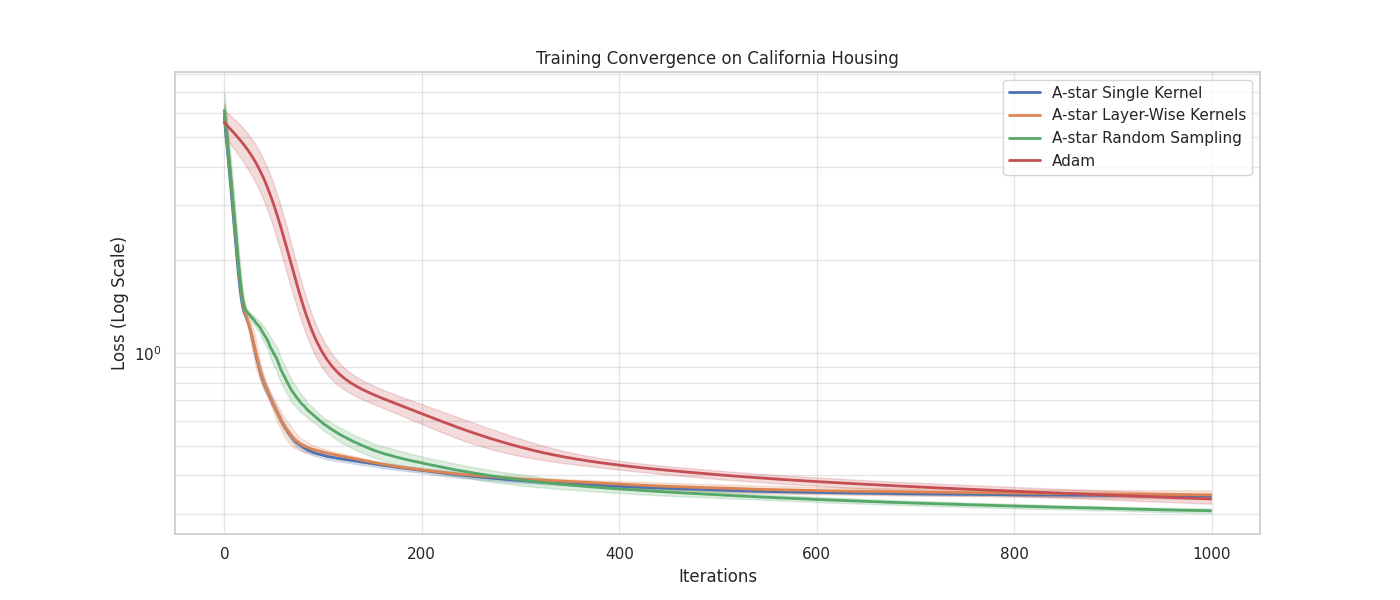
\includegraphics[width=1.1\textwidth]{figures/results/small_net_california_housing_Adam_vs_A-star/small_net_california_housing_Adam_vs_A-star_convergence.png}
    \caption{Small Net convergence: $A^*$ strategies vs. Adam on California Housing.}
    \label{fig:small_california_convergence}
\end{figure}

The convergence profiles reveal a notable performance advantage for stochastic search in low-parameter regimes. The \textit{$A^*$ Random Sampling} strategy (green line) demonstrates a superior ability to identify high-quality descent directions, ultimately reaching a final loss ($0.3075$) lower than the Adam baseline ($0.3358$). This suggests that the stochastic nature of $A^*$ effectively navigates the discrete error surface, avoiding local minima that can hinder gradient-based methods in constrained architectures.

The distribution of final loss values across 5 independent runs is visualized in Figure \ref{fig:small_california_final_loss}.

\begin{figure}[htbp]
    \centering
    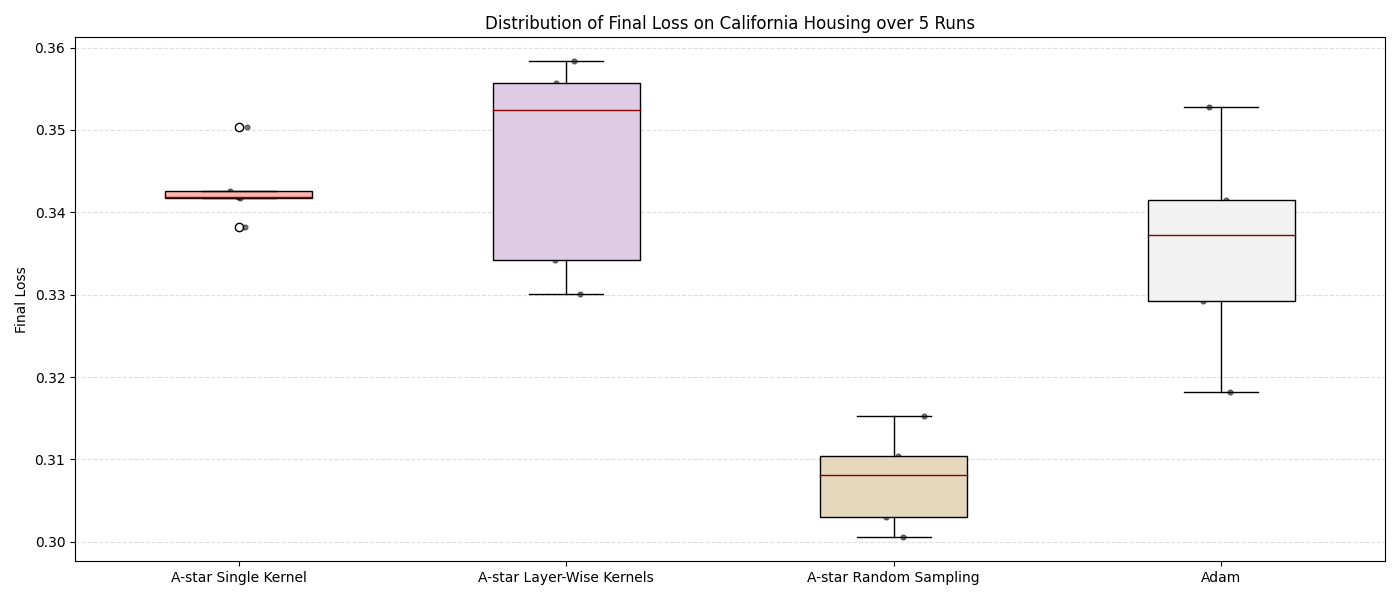
\includegraphics[width=1.0\textwidth]{figures/results/small_net_california_housing_Adam_vs_A-star/small_net_california_housing_Adam_vs_A-star_final_loss.png}
    \caption{Distribution of Final Loss for Small Net.}
    \label{fig:small_california_final_loss}
\end{figure}

The boxplot analysis confirms the reliability of the \textit{Random Sampling} strategy, which maintains a tight distribution with a median loss significantly below that of the kernel-based methods. While the \textit{Single Kernel} approach achieves lower accuracy, it exhibits the lowest standard deviation ($0.0040$), indicating high procedural consistency despite the restricted search space.


\subsubsection{Evaluation of Generalization Performance on the Test Set}
The predictive performance on unseen data is summarized in Figure \ref{fig:small_california_metrics_dist}.

\begin{figure}[htbp]
    \centering
    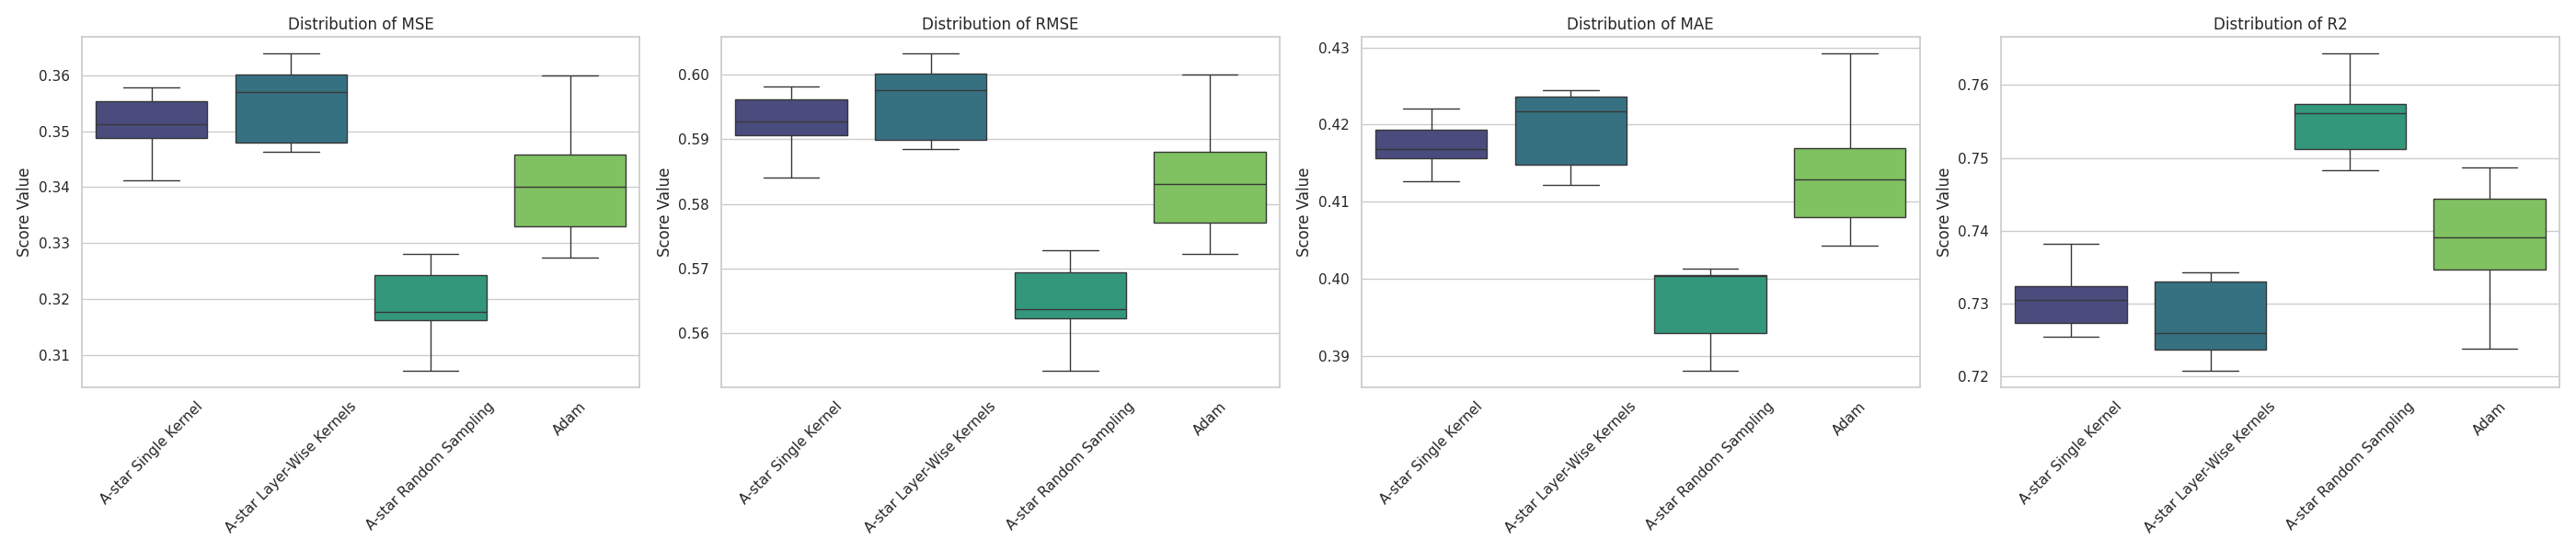
\includegraphics[width=1\textwidth]{figures/results/small_net_california_housing_Adam_vs_A-star/small_net_california_housing_Adam_vs_A-star_metrics_distribution.png}
    \caption{Regression metrics distribution (MSE, RMSE, MAE, $R^2$) across strategies for Small Net.}
    \label{fig:small_california_metrics_dist}
\end{figure}

The metric distributions confirm that \textit{Random Sampling} leads across all generalization categories. Specifically, it achieves a superior average $R^2$ of $0.7555$ and the lowest MSE ($0.3187$). Kernel-based methods cluster around an $R^2$ of $0.73$, suggesting that rigid geometric updates are less expressive than random perturbations in this specific architectural scale.

\subsubsection{Summary Statistics}

Table \ref{tab:small_net_california} provides the detailed numerical breakdown of the Small Net performance.

\begin{table}[htbp]
\centering
\scriptsize
\begin{tabular}{|l|c|c|c|c|}
\hline
\textbf{Metric}   & \textbf{$A^*$ Single Kernel} & \textbf{$A^*$ Layer-Wise} & \textbf{$A^*$ Random} & \textbf{Adam} \\ \hline
\multicolumn{5}{|l|}{\textit{Metrics computed on Training Set:}} \\ \hline
Avg Final Loss          & 0.3429                       & 0.3462                    & \textbf{0.3075}       & 0.3358        \\ 
Median Final Loss       & 0.3418                       & 0.3524                    & \textbf{0.3081}       & 0.3372        \\
Std Final Loss          & \textbf{0.0040}              & 0.0117                    & 0.0052                & 0.0117        \\ \hline
Avg Time (s)            & 2323.8644                    & 2319.0373                 & 307.9631              & \textbf{156.2262} \\ \hline
\multicolumn{5}{|l|}{\textit{Metrics computed on Test Set:}} \\ \hline
Avg MSE                 & 0.3509                       & 0.3551                    & \textbf{0.3187}       & 0.3413        \\ 
Avg RMSE                & 0.5923                       & 0.5959                    & \textbf{0.5645}       & 0.5841        \\ 
Avg MAE                 & 0.4173                       & 0.4194                    & \textbf{0.3966}       & 0.4143        \\ 
Avg $R^2$               & 0.7308                       & 0.7275                    & \textbf{0.7555}       & 0.7382        \\ \hline
\end{tabular}
\caption{Average statistical comparison on California Housing - Small Net.}
\label{tab:small_net_california}
\end{table}

The numerical results highlight that \textit{$A^*$ Random Sampling} not only outperformed the deterministic kernels but also achieved a higher $R^2$ ($0.7555$) than Adam ($0.7382$), establishing search as a viable alternative for small-scale regression tasks.

\newpage

\subsection{Medium Net Results}

\subsubsection{Visual Analysis of Training and Stability}

As the parameter space expands, the convergence dynamics shift, as shown in Figure \ref{fig:medium_california_convergence}.

\begin{figure}[htbp]
    \centering
    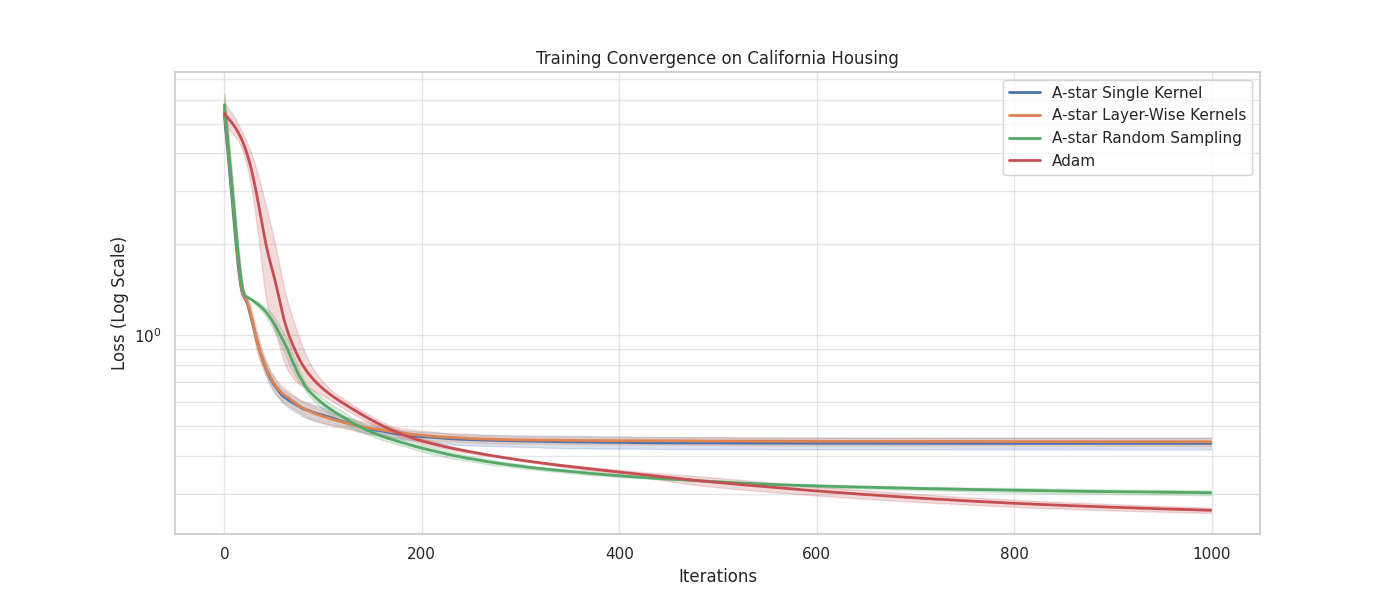
\includegraphics[width=1.1\textwidth]{figures/results/medium_net_california_housing_Adam_vs_A-star/medium_net_california_housing_Adam_vs_A-star_convergence.png}
    \caption{Medium Net convergence: $A^*$ strategies vs. Adam on California Housing}
    \label{fig:medium_california_convergence}
\end{figure}

In this intermediate scale, the efficiency of gradient-based optimization becomes apparent. Adam converges more rapidly and secures a lower loss plateau ($0.2642$). Among the $A^*$ variants, \textit{Random Sampling} remains the most effective search strategy, while kernel-based methods struggle to manage the increased dimensionality, plateauing at higher loss values.

\begin{figure}[H]
    \centering
    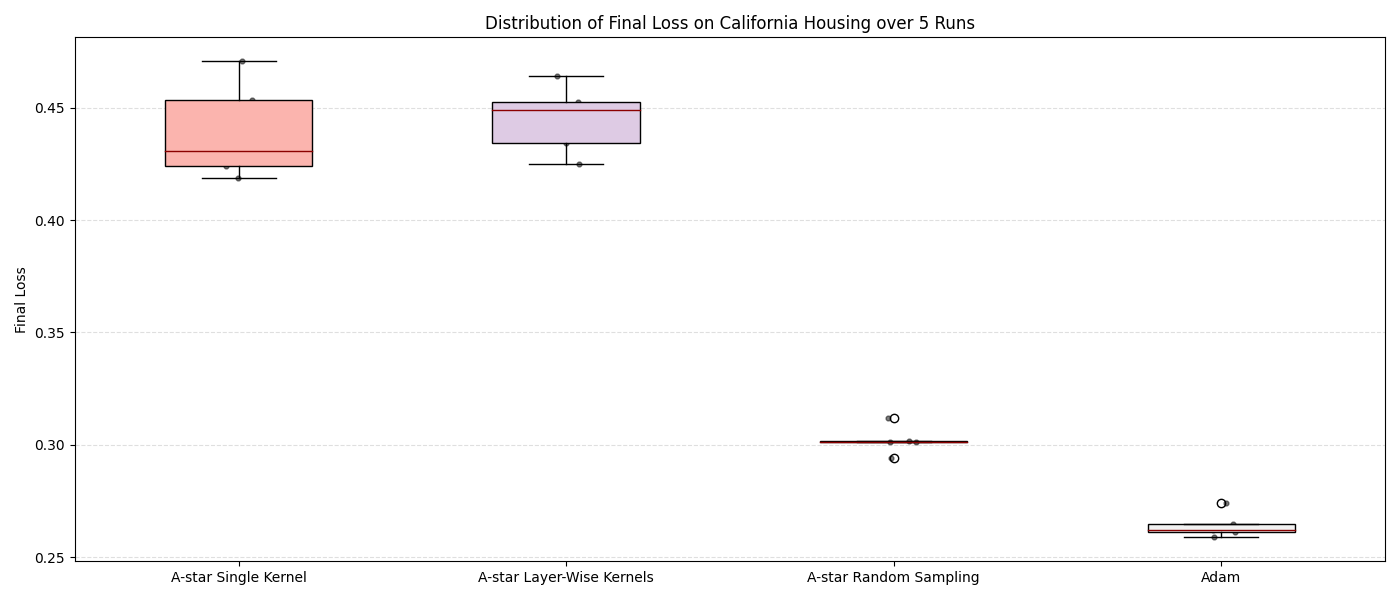
\includegraphics[width=1.0\textwidth]{figures/results/medium_net_california_housing_Adam_vs_A-star/medium_net_california_housing_Adam_vs_A-star_final_loss.png}
    \caption{Distribution of Final Loss for Medium Net.}
    \label{fig:medium_california_final_loss}
\end{figure}

The loss distribution emphasizes Adam's stability ($Std: 0.0054$). While \textit{$A^*$ Random Sampling} maintains competitive performance and low variance ($Std: 0.0057$), the kernel-based strategies exhibit significant performance degradation, highlighting the limitations of fixed-block neighbor generation in higher-dimensional weight spaces.


\subsubsection{Evaluation of Generalization Performance on the Test Set}
The test set results for the Medium Net are illustrated in Figure \ref{fig:medium_california_metrics_dist}.

\begin{figure}[htbp]
    \centering
    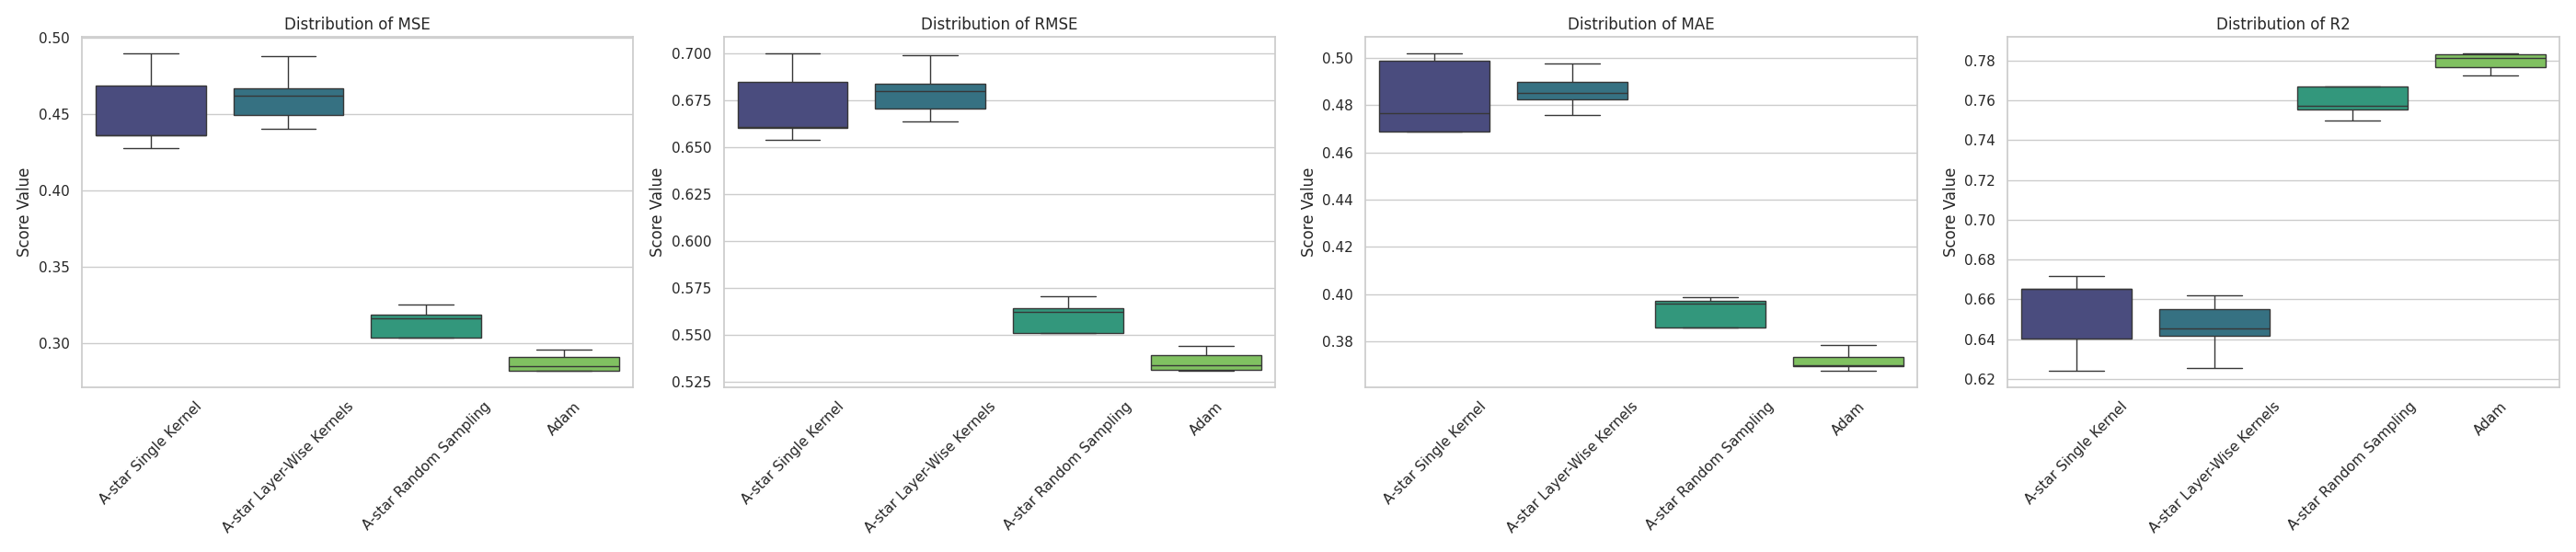
\includegraphics[width=1\textwidth]{figures/results/medium_net_california_housing_Adam_vs_A-star/medium_net_california_housing_Adam_vs_A-star_metrics_distribution.png}
    \caption{Regression metrics distribution across strategies for Medium Net.}
    \label{fig:medium_california_metrics_dist}
\end{figure}

The $R^2$ scores indicate that while Adam is the optimal performer ($0.7796$), \textit{$A^*$ Random Sampling} ($0.7593$) remains a robust search-based baseline. In contrast, the kernel methods show a notable drop in predictive power, with MSE exceeding $0.45$, suggesting that fixed-block updates are too restrictive for the error surfaces of medium-sized networks.

\subsubsection{Summary Statistics}

Table \ref{tab:medium_net_california} summarizes the Medium Net results.

\begin{table}[htbp]
\centering
\scriptsize
\begin{tabular}{|l|c|c|c|c|}
\hline
\textbf{Metric}   & \textbf{$A^*$ Single Kernel} & \textbf{$A^*$ Layer-Wise} & \textbf{$A^*$ Random} & \textbf{Adam} \\ \hline
\multicolumn{5}{|l|}{\textit{Metrics computed on Training Set:}} \\ \hline
Avg Final Loss          & 0.4395                       & 0.4450                    & 0.3021                & \textbf{0.2642} \\ 
Median Final Loss       & 0.4307                       & 0.4489                    & 0.3014                & \textbf{0.2622} \\
Std Final Loss          & 0.0196                       & 0.0138                    & 0.0057                & \textbf{0.0054} \\ \hline
Avg Time (s)            & 2069.8275                    & 2061.8664                 & 1044.4042             & \textbf{169.5691} \\ \hline
\multicolumn{5}{|l|}{\textit{Metrics computed on Test Set:}} \\ \hline
Avg MSE                 & 0.4520                       & 0.4616                    & 0.3137                & \textbf{0.2873} \\ 
Avg RMSE                & 0.6721                       & 0.6793                    & 0.5600                & \textbf{0.5360} \\ 
Avg MAE                 & 0.4831                       & 0.4861                    & 0.3928                & \textbf{0.3717} \\ 
Avg $R^2$               & 0.6532                       & 0.6458                    & 0.7593                & \textbf{0.7796} \\ \hline
\end{tabular}
\caption{Average statistical comparison on California Housing - Medium Net.}
\label{tab:medium_net_california}
\end{table}

While Adam maintains the performance lead, the $R^2$ of $0.7593$ achieved by \textit{$A^*$ Random Sampling} highlights the framework's sustained robustness even as the model's dimensionality increases.
\newpage

\subsection{Big Net Results}

\subsubsection{Visual Analysis of Training and Stability}

The convergence dynamics for the Big Net architecture are shown in Figure \ref{fig:big_california_convergence}. 

\begin{figure}[htbp]
    \centering
    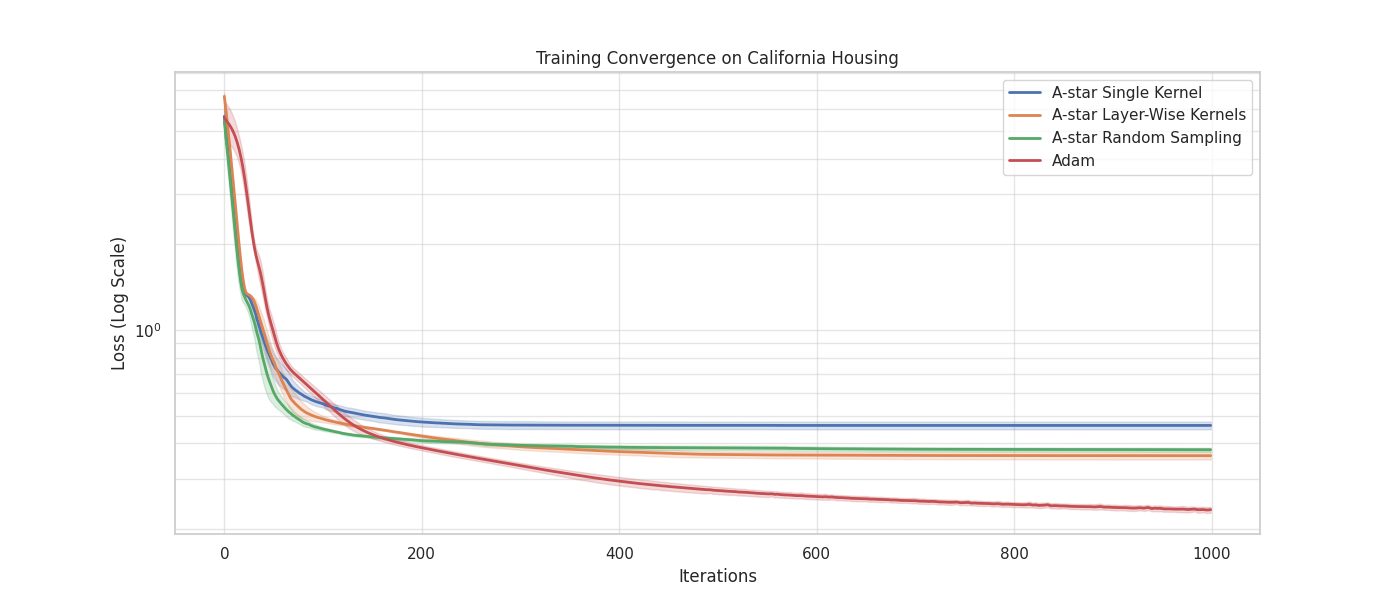
\includegraphics[width=1.1\textwidth]{figures/results/big_net_california_housing_Adam_vs_A-star/big_net_california_housing_Adam_vs_A-star_convergence.png}
    \caption{Big Net convergence: $A^*$ strategies vs. Adam on California Housing.}
    \label{fig:big_california_convergence}
\end{figure}

At this architectural scale, a "crossover" is observed: the \textit{$A^*$ Layer-Wise} strategy (orange line) begins to refine the loss more effectively than the \textit{Random Sampling} strategy. In this specific case, a structured approach to neighbor generation where kernel dimensions are tailored to specific network layers is more effective than purely stochastic sampling.

\begin{figure}[H]
    \centering
    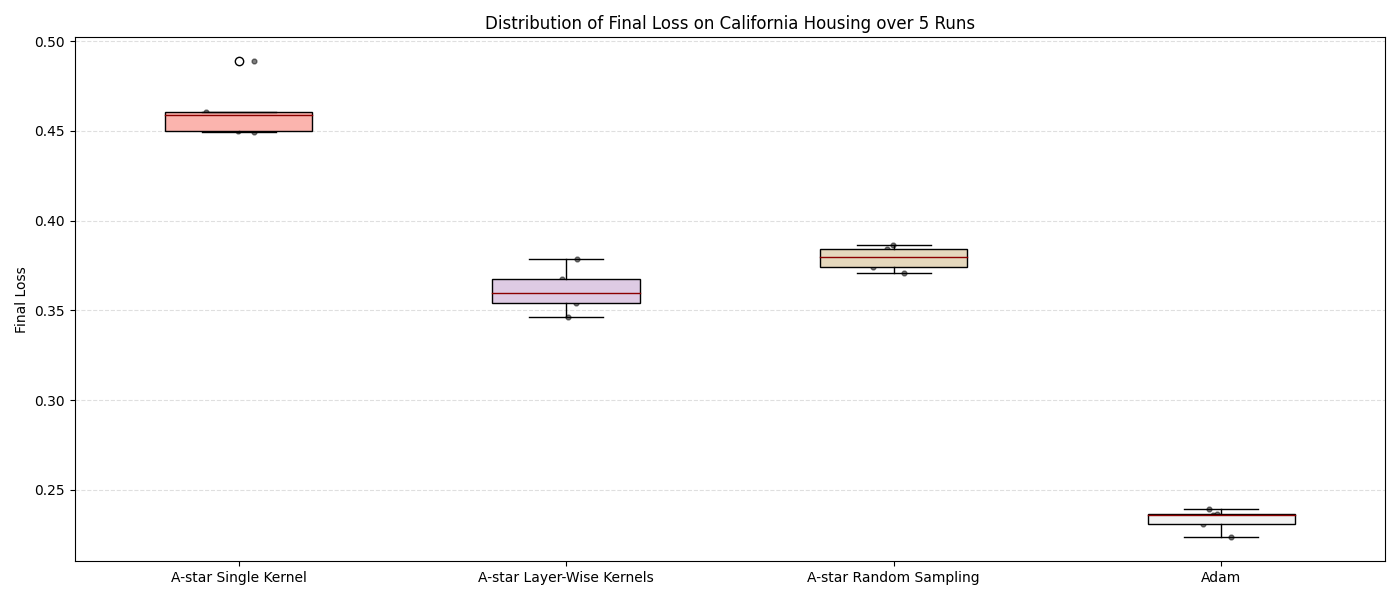
\includegraphics[width=1.0\textwidth]{figures/results/big_net_california_housing_Adam_vs_A-star/big_net_california_housing_Adam_vs_A-star_final_loss.png}
    \caption{Distribution of Final Loss for Big Net.}
    \label{fig:big_california_final_loss}
\end{figure}

Stability analysis reveals that Random Sampling and Adam maintain the lowest variance ($Std: 0.0059$ and $0.0056$). While the \textit{Layer-Wise} approach provides better final accuracy than Random search, it introduces slightly higher variability.


\subsubsection{Evaluation of Generalization Performance on the Test Set}
Generalization metrics for the Big Net are provided in Figure \ref{fig:big_california_metrics_dist}.

\begin{figure}[htbp]
    \centering
    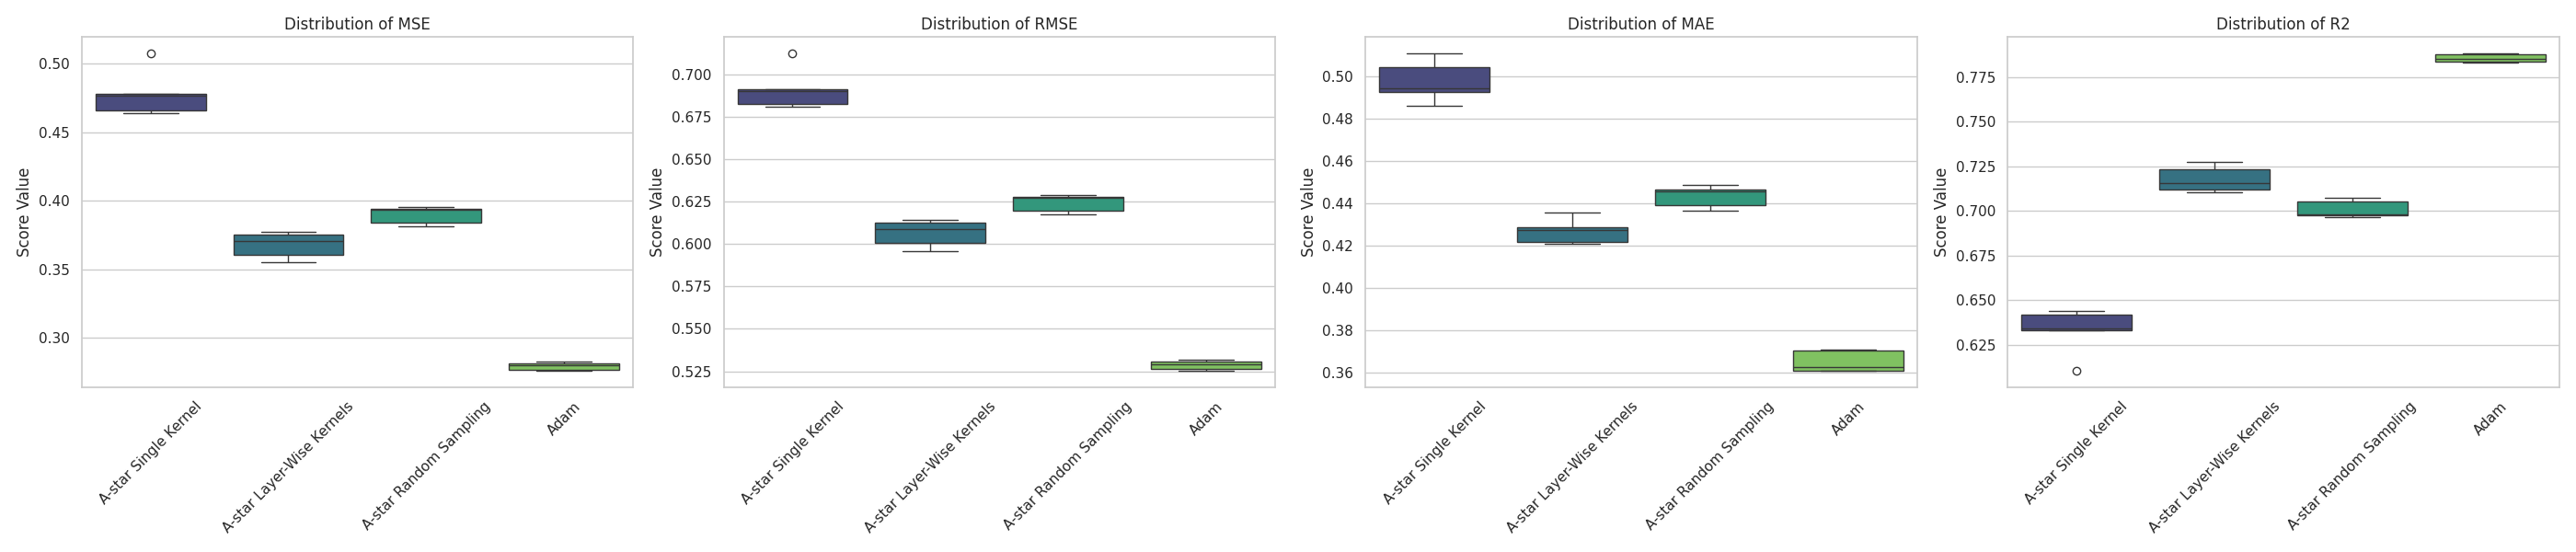
\includegraphics[width=1\textwidth]{figures/results/big_net_california_housing_Adam_vs_A-star/big_net_california_housing_Adam_vs_A-star_metrics_distribution.png}
    \caption{Regression metrics distribution across strategies for Big Net.}
    \label{fig:big_california_metrics_dist}
\end{figure}

The test data confirms the crossover effect; the Layer-Wise Kernel strategy achieves a superior $R^2$ ($0.7177$) compared to the Random strategy ($0.7011$). This suggests that structural awareness allows the $A^*$ search to exploit the hierarchical nature of the network more effectively as depth increases.

\subsubsection{Summary Statistics}

The following table presents the final numerical performance comparison for the Big Net.

\begin{table}[htbp]
\centering
\scriptsize
\begin{tabular}{|l|c|c|c|c|}
\hline
\textbf{Metric}   & \textbf{$A^*$ Single Kernel} & \textbf{$A^*$ Layer-Wise} & \textbf{$A^*$ Random} & \textbf{Adam} \\ \hline
\multicolumn{5}{|l|}{\textit{Metrics computed on Training Set:}} \\ \hline
Avg Final Loss          & 0.4615                       & 0.3612                    & 0.3791                & \textbf{0.2333} \\ 
Median Final Loss       & 0.4588                       & 0.3594                    & 0.3799                & \textbf{0.2361} \\
Std Final Loss          & 0.0144                       & 0.0112                    & 0.0059                & \textbf{0.0056} \\ \hline
Avg Time (s)            & 5735.2100                    & 10230.1885                & 7692.5054             & \textbf{194.4787} \\ \hline
\multicolumn{5}{|l|}{\textit{Metrics computed on Test Set:}} \\ \hline
Avg MSE                 & 0.4786                       & 0.3679                    & 0.3896                & \textbf{0.2794} \\ 
Avg RMSE                & 0.6917                       & 0.6065                    & 0.6242                & \textbf{0.5286} \\ 
Avg MAE                 & 0.4978                       & 0.4269                    & 0.4432                & \textbf{0.3650} \\ 
Avg $R^2$               & 0.6328                       & 0.7177                    & 0.7011                & \textbf{0.7856} \\ \hline
\end{tabular}
\caption{Average statistical comparison on California Housing - Big Net.}
\label{tab:big_net_california}
\end{table}

While Adam remains the standard for efficiency, the Layer-Wise $A^*$ approach emerges as a challenger; it represents the most scalable search-based alternative for deep architectures, effectively narrowing the performance gap as complexity increases.
\subsection{Conclusions on California Housing Benchmark}

The multi-scale analysis provides several key insights:

\begin{itemize}
    \item \textbf{Search-Based Optimization Potential:} In the Small Net, $A^*$ with Random Sampling outperformed Adam in $R^2$ ($0.7555$ vs $0.7382$), proving that discrete search can surpass local gradient descent in low-parameter spaces.
    \item \textbf{A-Star Methods Scaling:} A "strategy crossover" occurs between Medium and Big Nets; while Random Sampling is optimal for smaller architectures, the Layer-Wise Kernel strategy is significantly more effective as network complexity grows.
    \item \textbf{Computational Efficiency:} Adam maintains a decisive advantage in execution speed, especially as network size increases, due to the inherent computational overhead of exploring discretized neighborhood states.
\end{itemize}




%==============================================================================================================================================
%=============================================               SINE FUNCTION             ========================================================
%==============================================================================================================================================

\newpage

\section{Noisy Sine Function Regression}
\label{sec:results_sine}

The Noisy Sine benchmark evaluates the capacity of the $A^*$ search framework to model non-linear periodic functions under the influence of Gaussian noise. This task specifically tests the precision of neighbor generation strategies in a low-dimensional space.

\subsection{Small Net Results}

\subsubsection{Visual Analysis of Training and Stability}

The convergence behavior for the Small Net on the Noisy Sine task is depicted in Figure \ref{fig:small_sine_convergence}. 

\begin{figure}[htbp]
    \centering
    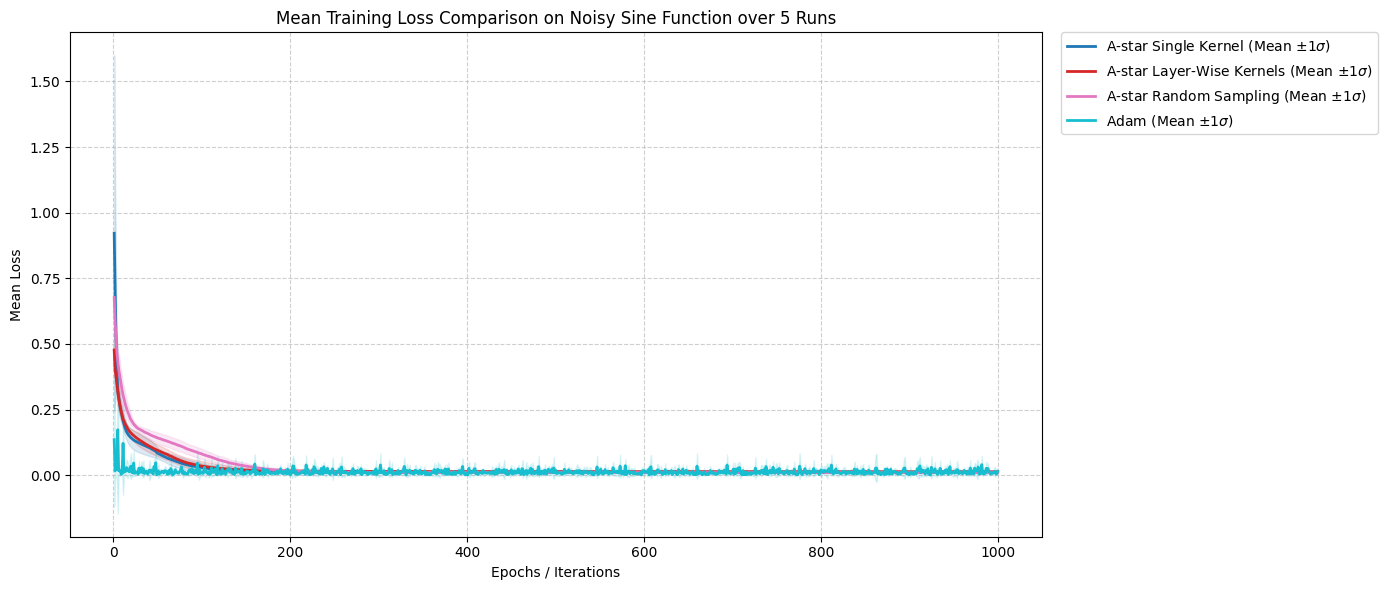
\includegraphics[width=1.1\textwidth]{figures/results/small_net_sine_Adam_vs_A-star/small_net_sine_Adam_vs_A-star_mean_loss.png}
    \caption{Small Net convergence: $A^*$ strategies vs. Adam on Noisy Sine.}
    \label{fig:small_sine_convergence}
\end{figure}

The convergence profiles indicate that for small-scale architectures, stochastic search effectively competes with gradient-based methods. While the Adam baseline converges rapidly to a high-quality local minimum in the early stages of training, it subsequently exhibits persistent oscillations around this point, failing to refine the solution further. In contrast, the \textit{$A^*$ Random Sampling} strategy demonstrates a superior ability to identify global parameters, reaching an average final loss of $0.0098$, which is notably lower than Adam's $0.0147$. This suggests that while gradient descent excels at initial descent, the discrete exploration of $A^*$ can bypass local plateaus and refine weights beyond the point where standard optimizers stall.
The distribution of final loss values across 5 independent runs is visualized in Figure \ref{fig:small_sine_final_loss}.

\begin{figure}[htbp]
    \centering
    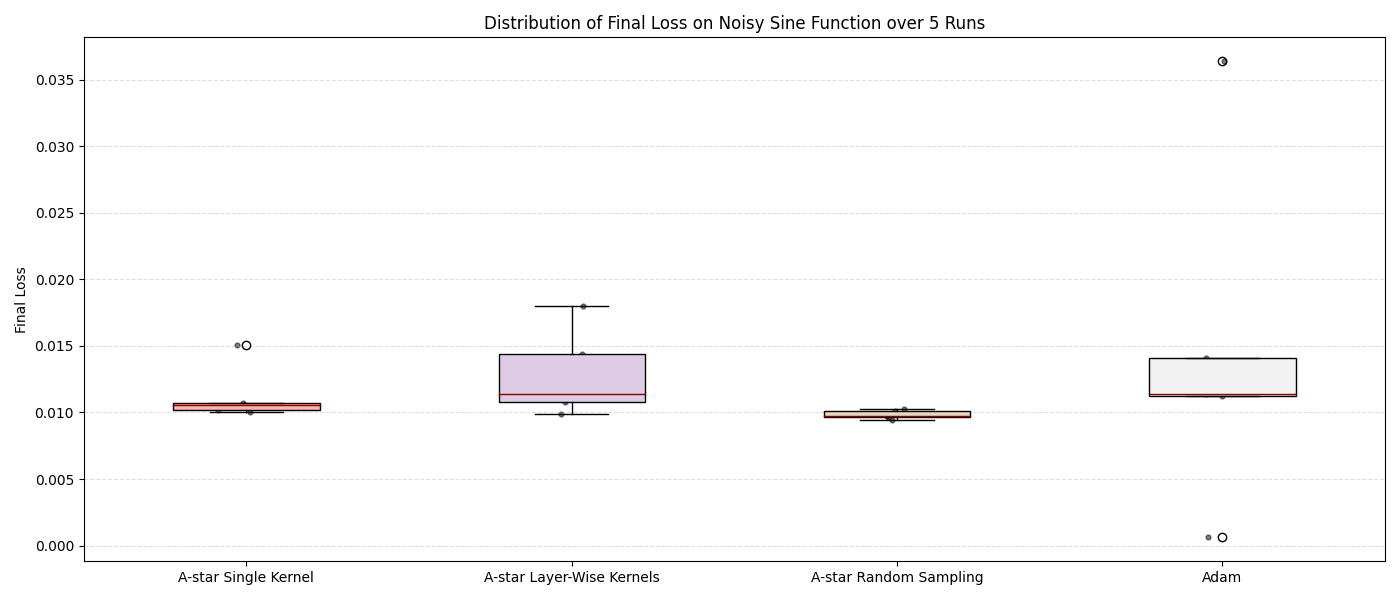
\includegraphics[width=1.0\textwidth]{figures/results/small_net_sine_Adam_vs_A-star/small_net_sine_Adam_vs_A-star_final_loss.png}
    \caption{Distribution of Final Loss for Small Net.}
    \label{fig:small_sine_final_loss}
\end{figure}

The stability analysis reveals that \textit{Random Sampling} is exceptionally consistent, showing the lowest standard deviation ($0.0003$). In contrast, Adam shows significantly higher standard deviation ($0.0118$) in this regime, indicating that gradient descent is more sensitive to initialization when the network capacity is limited.


\subsubsection{Evaluation of Generalization Performance on the Test Set}
The predictive performance on unseen data is summarized in Figure \ref{fig:small_sine_metrics_dist}.

\begin{figure}[htbp]
    \centering
    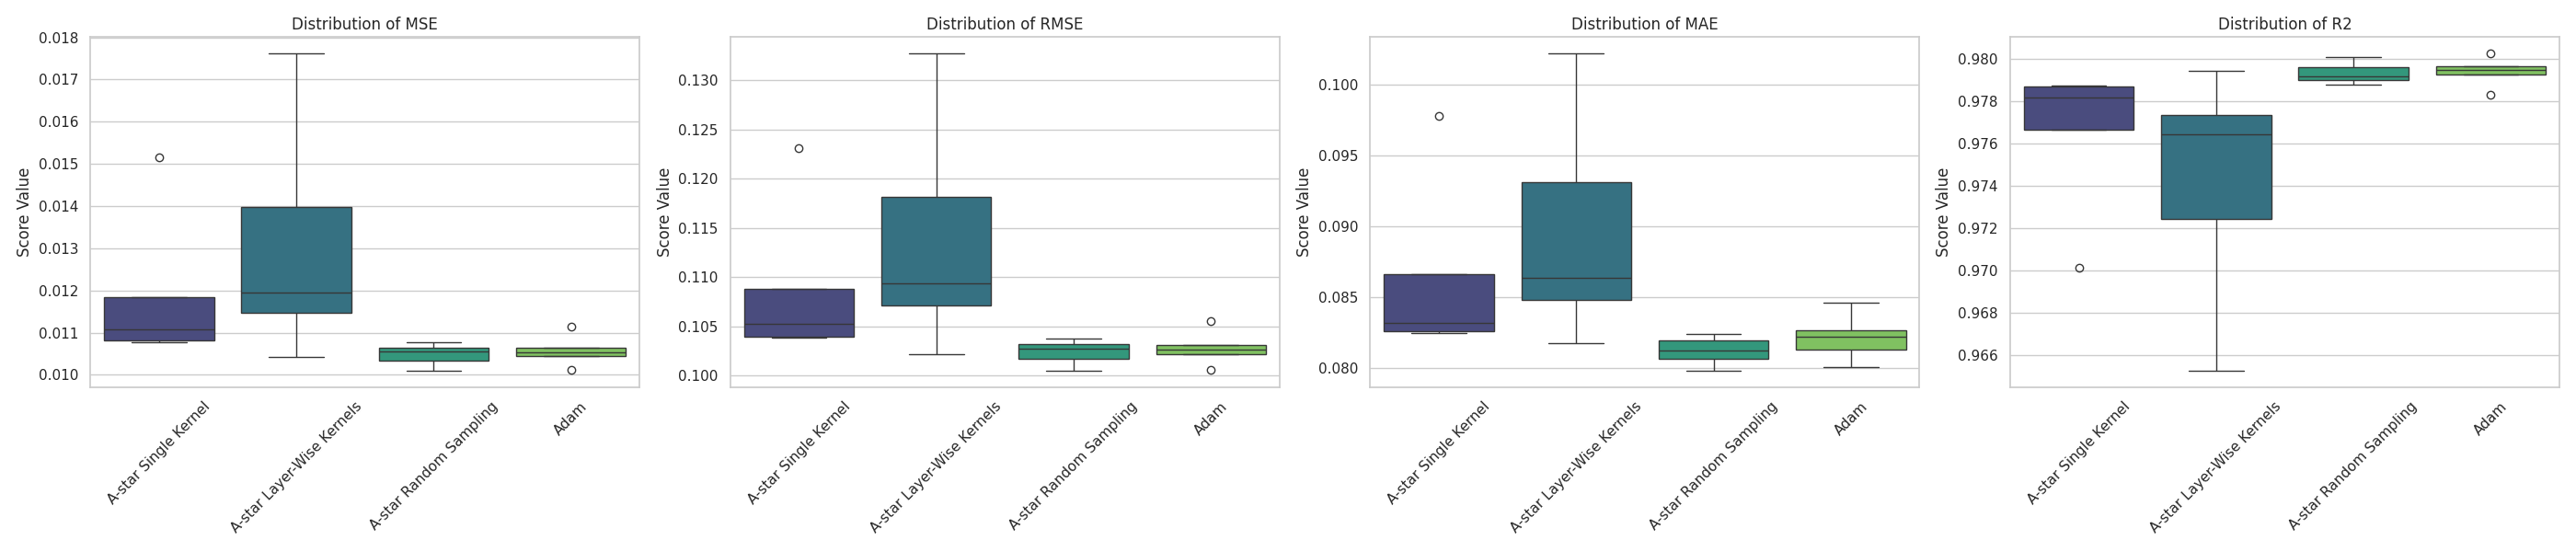
\includegraphics[width=1.05\textwidth]{figures/results/small_net_sine_Adam_vs_A-star/small_net_sine_Adam_vs_A-star_metrics_distribution.png}
    \caption{Regression metrics distribution (MSE, RMSE, MAE, $R^2$) across strategies for Small Net.}
    \label{fig:small_sine_metrics_dist}
\end{figure}

Generalization metrics confirm the dominance of \textit{Random Sampling} in the small-scale regime. It achieved a superior average MSE of $0.0105$, outperforming the other search variants. Both Random Sampling and Adam achieved $R^2$ values exceeding $0.979$, demonstrating that the search framework is fully capable of capturing underlying periodicity despite injected noise.

\subsubsection{Summary Statistics}

Table \ref{tab:small_net_sine} provides the detailed numerical breakdown of the Small Net performance.

\begin{table}[htbp]
\centering
\scriptsize
\begin{tabular}{|l|c|c|c|c|}
\hline
\textbf{Metric}   & \textbf{$A^*$ Single Kernel} & \textbf{$A^*$ Layer-Wise} & \textbf{$A^*$ Random} & \textbf{Adam} \\ \hline
\multicolumn{5}{|l|}{\textit{Metrics computed on Training Set:}} \\ \hline
Avg Final Loss          & 0.0113                       & 0.0129                    & \textbf{0.0098}       & 0.0147        \\ 
Median Final Loss       & 0.0106                       & 0.0114                    & \textbf{0.0097}       & 0.0114        \\
Std Final Loss          & 0.0019                       & 0.0030                    & \textbf{0.0003}       & 0.0118        \\ \hline
Avg Time (s)            & 1194.7349                    & 1225.2439                 & \textbf{178.7269}     & 782.8654      \\ \hline
\multicolumn{5}{|l|}{\textit{Metrics computed on Test Set:}} \\ \hline
Avg MSE                 & 0.0119                       & 0.0131                    & \textbf{0.0105}       & 0.0106        \\ 
Avg RMSE                & 0.1090                       & 0.1139                    & \textbf{0.1024}       & 0.1028        \\ 
Avg MAE                 & 0.0865                       & 0.0896                    & \textbf{0.0812}       & 0.0822        \\ 
Avg $R^2$               & 0.9765                       & 0.9742                    & 0.9793                & \textbf{0.9794} \\ \hline
\end{tabular}
\caption{Average statistical comparison on Noisy Sine - Small Net.}
\label{tab:small_net_sine}
\end{table}

\newpage

\subsection{Medium Net Results}

\subsubsection{Visual Analysis of Training and Stability}

As the model capacity increases, the convergence dynamics for the Medium Net are shown in Figure \ref{fig:medium_sine_convergence}.

\begin{figure}[htbp]
    \centering
    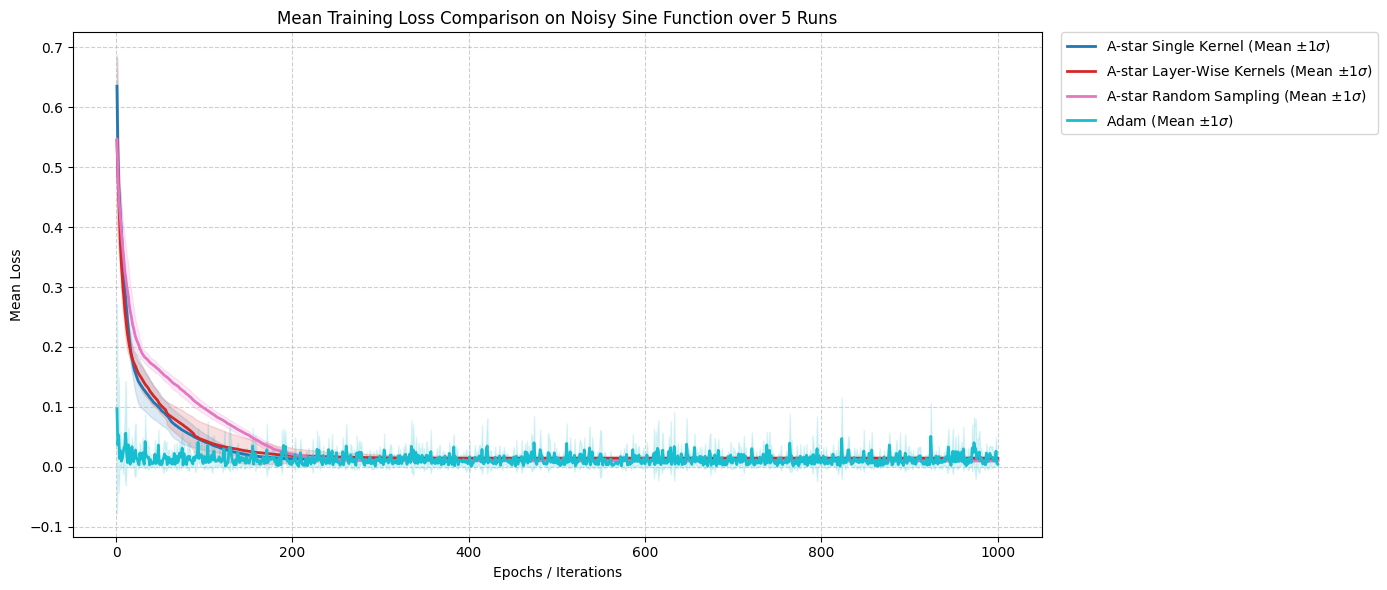
\includegraphics[width=1.1\textwidth]{figures/results/medium_net_sine_Adam_vs_A-star/medium_net_sine_Adam_vs_A-star_mean_loss.png}
    \caption{Medium Net convergence: $A^*$ strategies vs. Adam on Noisy Sine.}
    \label{fig:medium_sine_convergence}
\end{figure}

In the Medium Net, Adam exhibits its characteristic efficiency, rapidly descending to a high-quality local minimum within the first few iterations. However, following this initial descent, the optimizer tends to oscillate with high frequency around the identified minimum, struggling to achieve further refinement. Despite this, Adam secures the lowest average final loss ($0.0042$). Meanwhile, \textit{$A^*$ Random Sampling} remains a potent contender, maintaining a steady and stable trajectory to reach a loss of $0.0096$, significantly outperforming the kernel-based variants.

\begin{figure}[H]
    \centering
    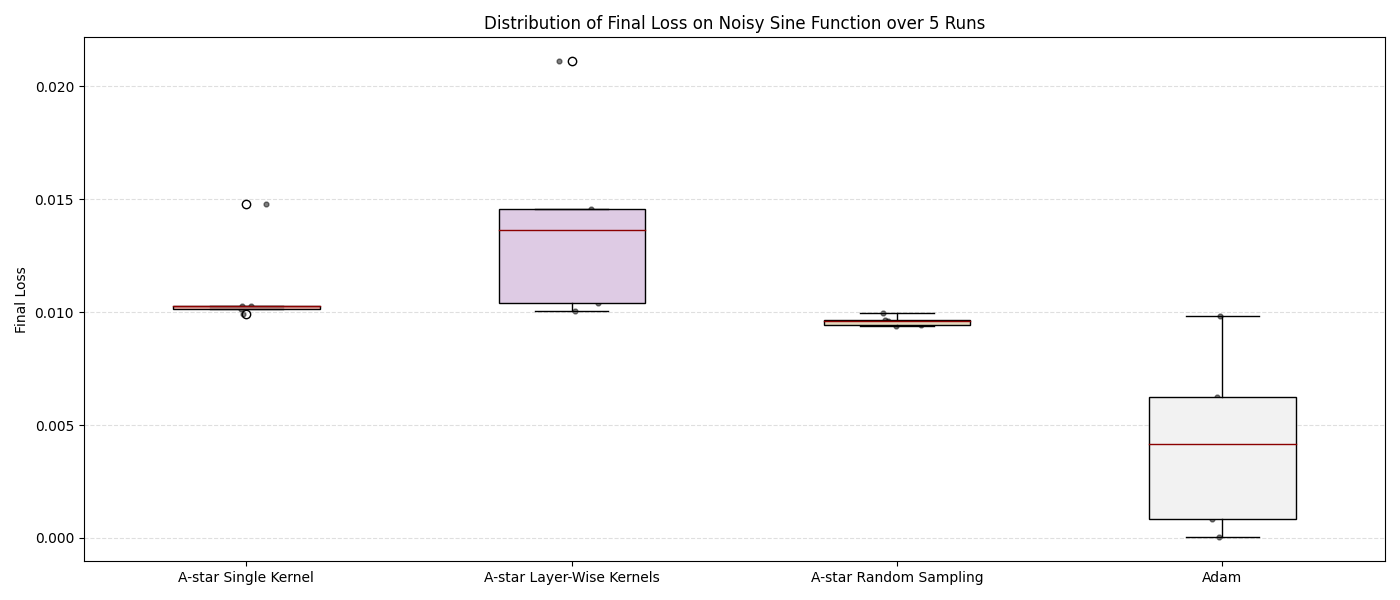
\includegraphics[width=1.0\textwidth]{figures/results/medium_net_sine_Adam_vs_A-star/medium_net_sine_Adam_vs_A-star_final_loss.png}
    \caption{Distribution of Final Loss for Medium Net.}
    \label{fig:medium_sine_final_loss}
\end{figure}

Stability analysis shows that \textit{Random Sampling} remains the most stable search method ($Std: 0.0002$). While Adam reaches a lower minimum, it exhibits higher variance ($Std: 0.0036$) across independent runs compared to the search-based sampling approach.


\subsubsection{Evaluation of Generalization Performance on the Test Set}
Generalization results for the Medium Net are illustrated in Figure \ref{fig:medium_sine_metrics_dist}.

\begin{figure}[htbp]
    \centering
    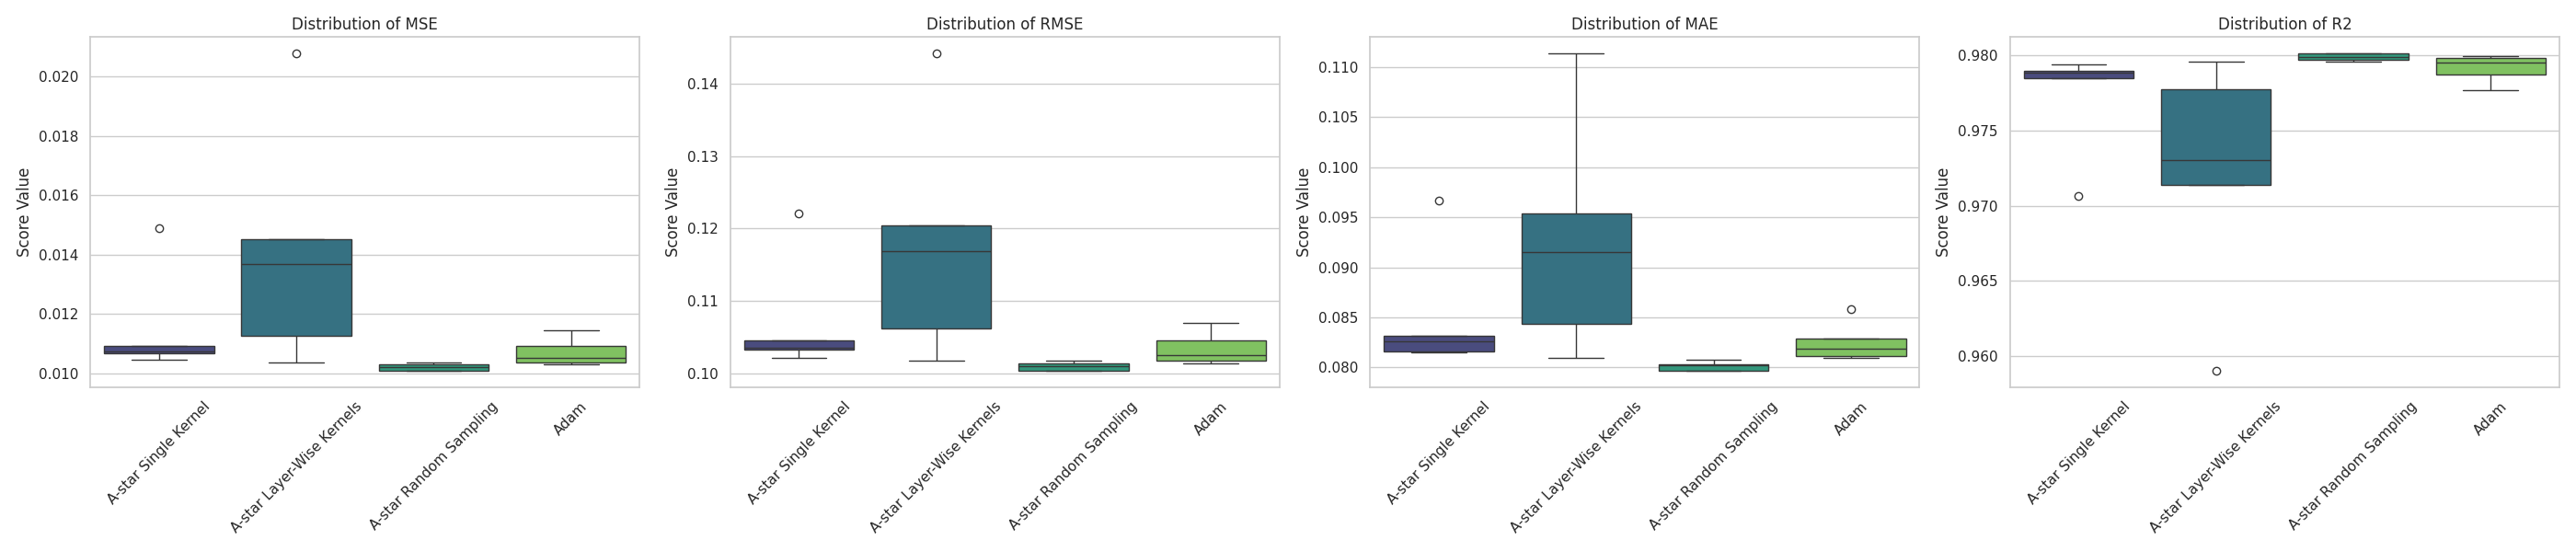
\includegraphics[width=1\textwidth]{figures/results/medium_net_sine_Adam_vs_A-star/medium_net_sine_Adam_vs_A-star_metrics_distribution.png}
    \caption{Regression metrics distribution across strategies for Medium Net.}
    \label{fig:medium_sine_metrics_dist}
\end{figure}

An interesting observation occurs in the test metrics: despite Adam reaching lower training losses through rapid initial descent, \textit{$A^*$ Random Sampling} achieved a superior average MSE ($0.0102$) and $R^2$ ($0.9799$) on unseen data.
\subsubsection{Summary Statistics}

Table \ref{tab:medium_net_sine} summarizes the results for the Medium Net.

\begin{table}[htbp]
\centering
\scriptsize
\begin{tabular}{|l|c|c|c|c|}
\hline
\textbf{Metric}   & \textbf{$A^*$ Single Kernel} & \textbf{$A^*$ Layer-Wise} & \textbf{$A^*$ Random} & \textbf{Adam} \\ \hline
\multicolumn{5}{|l|}{\textit{Metrics computed on Training Set:}} \\ \hline
Avg Final Loss          & 0.0111                       & 0.0140                    & 0.0096                & \textbf{0.0042} \\ 
Median Final Loss       & 0.0103                       & 0.0136                    & 0.0096                & \textbf{0.0042} \\
Std Final Loss          & 0.0019                       & 0.0040                    & \textbf{0.0002}       & 0.0036        \\ \hline
Avg Time (s)            & 1033.8106                    & 1079.9212                 & \textbf{503.6809}     & 1028.1696     \\ \hline
\multicolumn{5}{|l|}{\textit{Metrics computed on Test Set:}} \\ \hline
Avg MSE                 & 0.0115                       & 0.0141                    & \textbf{0.0102}       & 0.0107        \\ 
Avg RMSE                & 0.1071                       & 0.1179                    & \textbf{0.1010}       & 0.1034        \\ 
Avg MAE                 & 0.0851                       & 0.0927                    & \textbf{0.0801}       & 0.0825        \\ 
Avg $R^2$               & 0.9773                       & 0.9722                    & \textbf{0.9799}       & 0.9791        \\ \hline
\end{tabular}
\caption{Average statistical comparison on Noisy Sine - Medium Net.}
\label{tab:medium_net_sine}
\end{table}

\newpage

\subsection{Big Net Results}

\subsubsection{Visual Analysis of Training and Stability}

The convergence dynamics for the Big Net architecture are shown in Figure \ref{fig:big_sine_convergence}.

\begin{figure}[htbp]
    \centering
    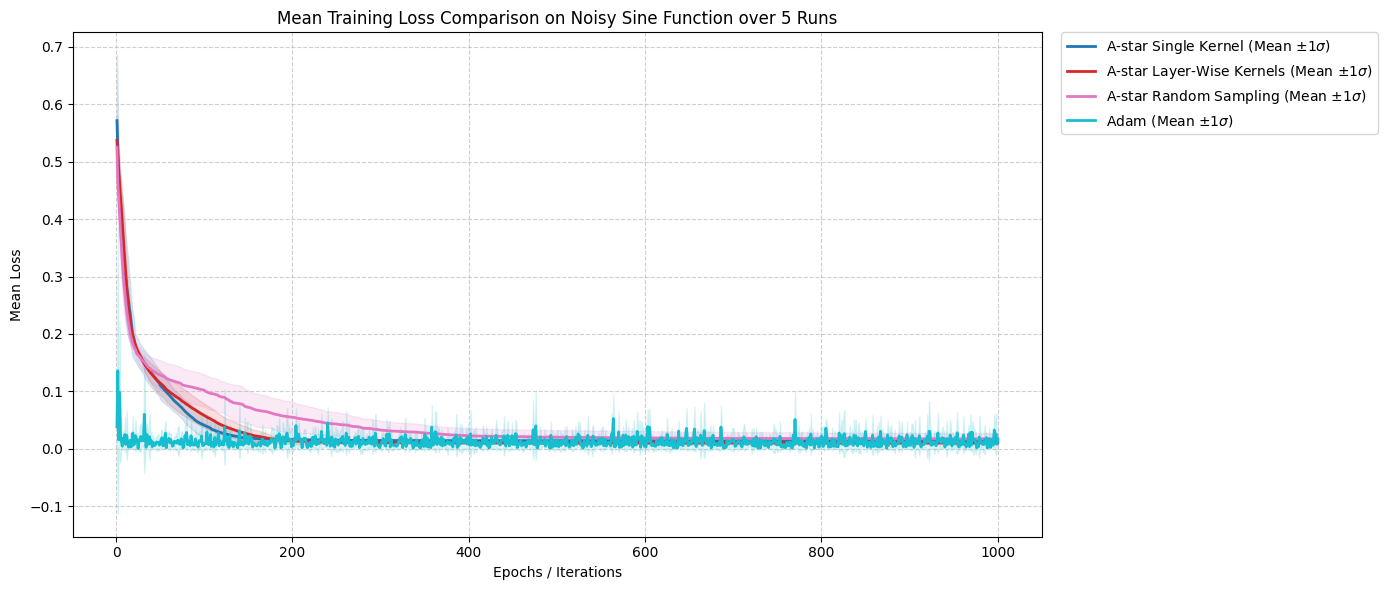
\includegraphics[width=1.1\textwidth]{figures/results/big_net_sine_Adam_vs_A-star/big_net_sine_Adam_vs_A-star_mean_loss.png}
    \caption{Big Net convergence: $A^*$ strategies vs. Adam on Noisy Sine.}
    \label{fig:big_sine_convergence}
\end{figure}

In the Big Net regime, a strategic "crossover" occurs: the \textit{$A^*$ Layer-Wise} strategy (orange line) emerges as a formidable challenger, outperforming all other search variants to reach a training loss of $0.0102$. While Adam is capable of reaching the absolute lowest training minimum ($0.0015$) through rapid initial descent, it exhibits significant convergence instability in this high-parameter space; after the early iterations, it typically begins to oscillate with high frequency and high variance around the local minima. Consequently, Adam's average performance ($0.0172$) is hindered by these volatile dynamics, whereas the Layer-Wise search remains remarkably consistent, providing a stable and scalable alternative for deep architectures.

\begin{figure}[H]
    \centering
    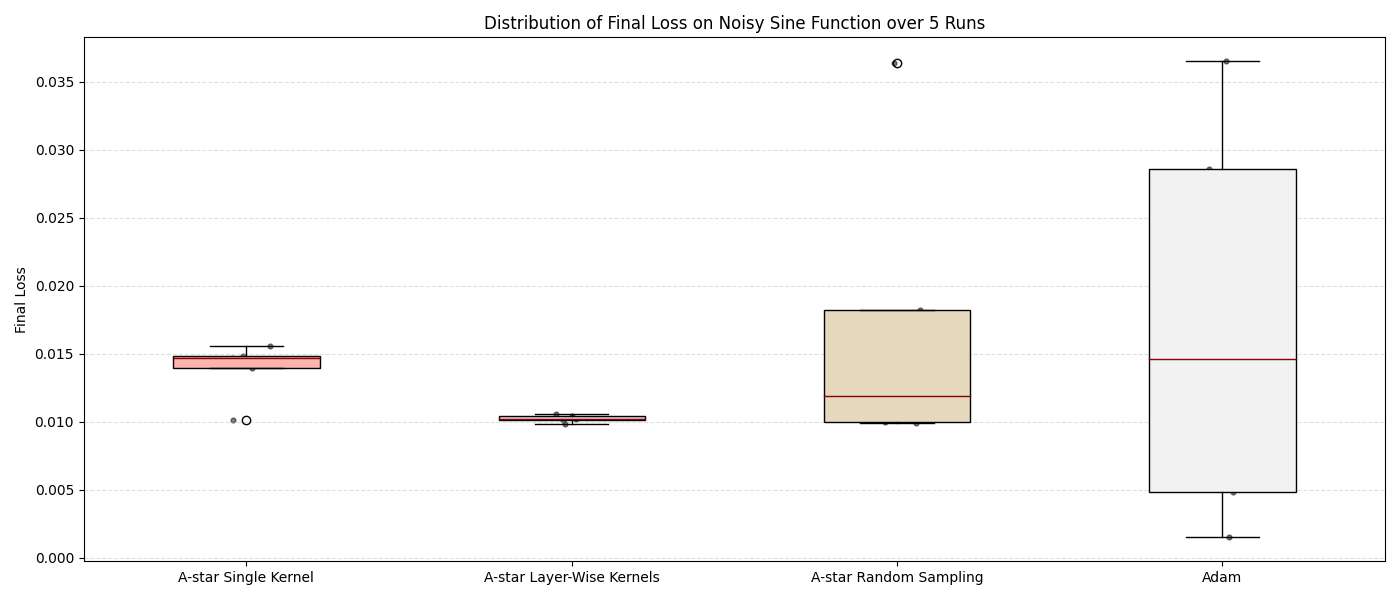
\includegraphics[width=1.0\textwidth]{figures/results/big_net_sine_Adam_vs_A-star/big_net_sine_Adam_vs_A-star_final_loss.png}
    \caption{Distribution of Final Loss for Big Net.}
    \label{fig:big_sine_final_loss}
\end{figure}

Stability analysis confirms that \textit{Layer-Wise Kernels} provide the most reliable search-based optimization for Big Nets ($Std: 0.0003$). Both \textit{Random Sampling} and Adam exhibit significantly higher variability ($Std: 0.0100$ and $0.0135$ respectively).


\subsubsection{Evaluation of Generalization Performance on the Test Set}
Generalization metrics for the Big Net are provided in Figure \ref{fig:big_sine_metrics_dist}.

\begin{figure}[htbp]
    \centering
    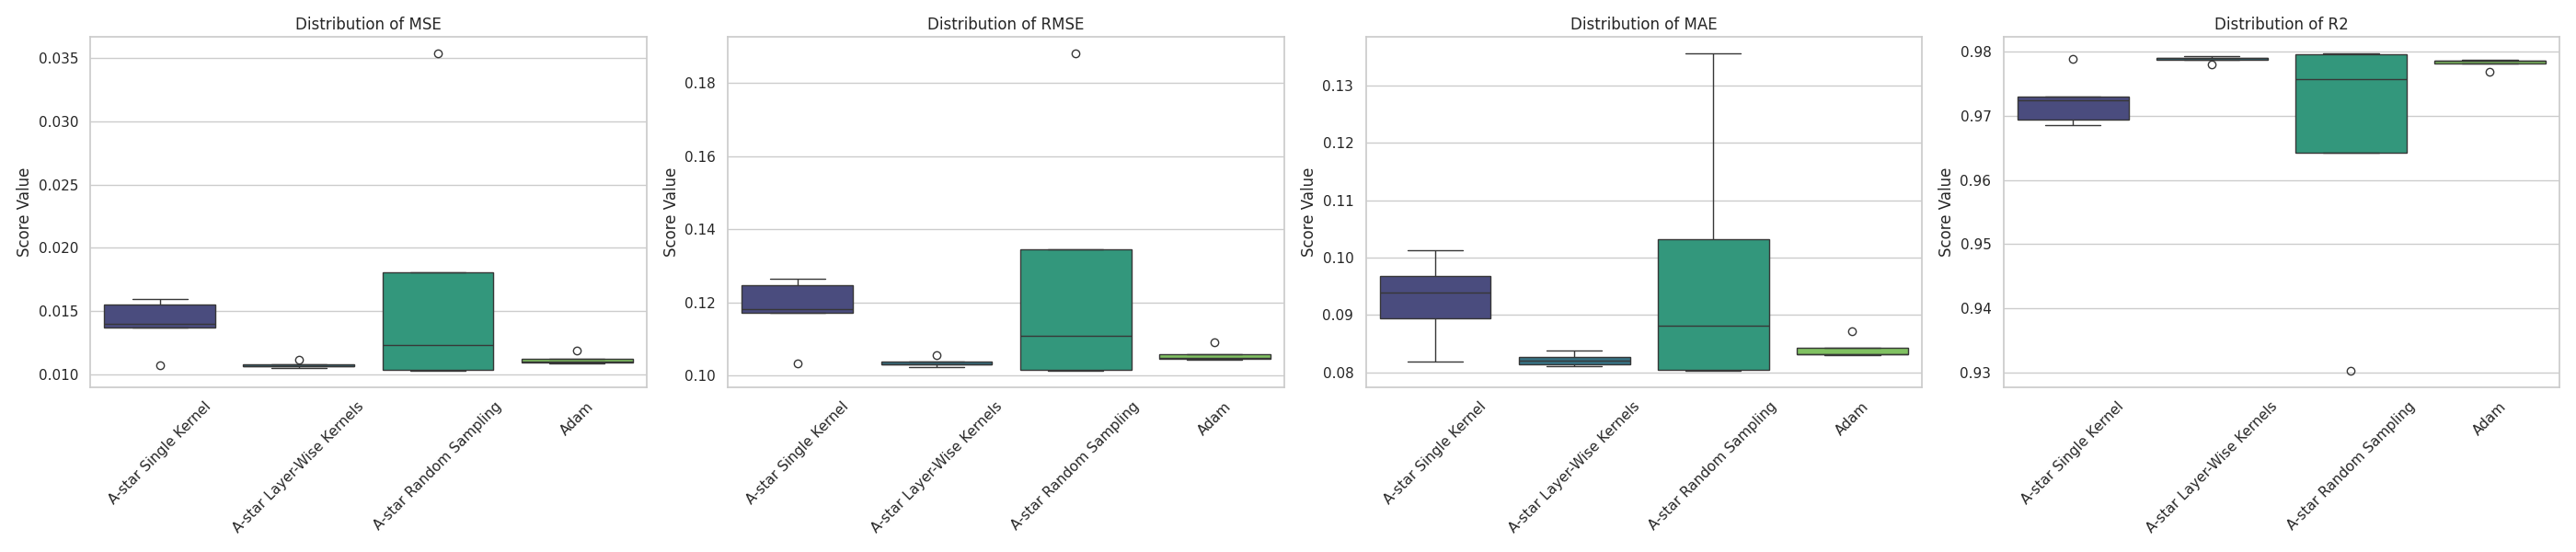
\includegraphics[width=1.05\textwidth]{figures/results/big_net_sine_Adam_vs_A-star/big_net_sine_Adam_vs_A-star_metrics_distribution.png}
    \caption{Regression metrics distribution across strategies for Big Net.}
    \label{fig:big_sine_metrics_dist}
\end{figure}

The test data underscores the crossover effect: the \textit{Layer-Wise} strategy achieves a superior $R^2$ ($0.9788$) and the lowest MSE ($0.0107$) among all methods, including Adam. This reinforces the hypothesis that structured kernel updates become essential for search-based optimization as network depth increases.

\subsubsection{Summary Statistics}

The table below presents the numerical comparison for the Big Net.

\begin{table}[H]
\centering
\scriptsize
\begin{tabular}{|l|c|c|c|c|}
\hline
\textbf{Metric}   & \textbf{$A^*$ Single Kernel} & \textbf{$A^*$ Layer-Wise} & \textbf{$A^*$ Random} & \textbf{Adam} \\ \hline
\multicolumn{5}{|l|}{\textit{Metrics computed on Training Set:}} \\ \hline
Avg Final Loss          & 0.0138                       & \textbf{0.0102}           & 0.0173                & 0.0172        \\ 
Median Final Loss       & 0.0147                       & \textbf{0.0102}           & 0.0119                & 0.0146        \\
Std Final Loss          & 0.0019                       & \textbf{0.0003}           & 0.0100                & 0.0135        \\ \hline
Avg Time (s)            & 2224.3329                    & 3054.9725                 & 2873.0685             & \textbf{1565.1961} \\ \hline
\multicolumn{5}{|l|}{\textit{Metrics computed on Test Set:}} \\ \hline
Avg MSE                 & 0.0140                       & \textbf{0.0107}           & 0.0173                & 0.0112        \\ 
Avg RMSE                & 0.1180                       & \textbf{0.1036}           & 0.1273                & 0.1058        \\ 
Avg MAE                 & 0.0927                       & \textbf{0.0822}           & 0.0975                & 0.0842        \\ 
Avg $R^2$               & 0.9724                       & \textbf{0.9788}           & 0.9659                & 0.9782        \\ \hline
\end{tabular}
\caption{Average statistical comparison on Noisy Sine - Big Net.}
\label{tab:big_net_sine}
\end{table}

\subsection{Conclusions on Noisy Sine Benchmark}

The analysis of the Noisy Sine benchmark reveals several key insights:

\begin{itemize}
    \item \textbf{Search-Based Precision:} In Small and Medium Nets, $A^*$ search (specifically Random Sampling) achieved generalization metrics that matched or exceeded Adam, proving its efficacy in periodic regression.
    \item \textbf{Adaptive Crossover Law:} The "strategy crossover" is once again confirmed; while Random Sampling is optimal for smaller models, the \textbf{Layer-Wise Kernel} strategy is the only search variant that maintains stability and performance in the Big Net.
    \item \textbf{Robustness to Noise:} The search framework exhibits high resilience to noise, achieving lower test-set variance than Adam in several cases, suggesting a natural resistance to overfitting in periodic tasks.
\end{itemize}


%==============================================================================================================================================
%=============================================               IRIS FLOWER               ========================================================
%==============================================================================================================================================

\newpage

\section{Iris Flower Classification}
\label{sec:results_iris}

The Iris Flower benchmark evaluates the $A^*$ search framework's efficacy in a multi-class classification context. Unlike the continuous regression of the Sine task, this benchmark requires the optimizers to establish clear decision boundaries between three distinct species (Setosa, Versicolor, and Virginica) based on four morphological features.

\subsection{Small Net Results}

\subsubsection{Visual Analysis of Training and Stability}

The convergence behavior for the Small Net on the Iris task is depicted in Figure \ref{fig:small_iris_convergence}. 

\begin{figure}[htbp]
    \centering
    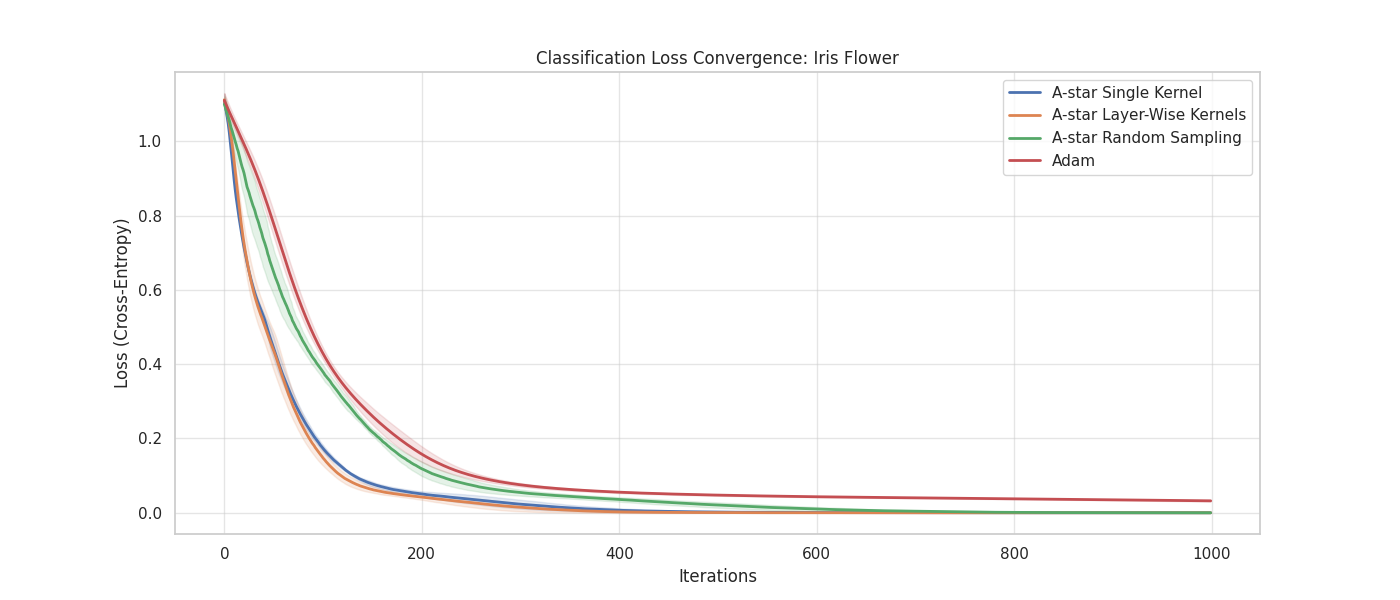
\includegraphics[width=1.1\textwidth]{figures/results/small_net_iris_Adam_vs_A-star/small_net_iris_Adam_vs_A-star_loss_convergence.png}
    \caption{Small Net convergence: $A^*$ strategies vs. Adam on Iris Flower.}
    \label{fig:small_iris_convergence}
\end{figure}

The convergence profiles highlight a remarkable performance by the search framework. The Adam baseline decreases the loss smoothly; however, it exhibits a much shallower trajectory compared to the search-based methods, settling at an average loss of $0.0322$. Adam behaves similarly to the \textit{$A^*$ Random Sampling} method, with both showing a slower, gradual convergence phase. In contrast, the kernel-based strategies, specifically \textit{Single Kernel} and \textit{Layer-Wise Kernels} demonstrate the steepest descent slopes, converging faster to much deeper local minima. \textit{$A^*$ Layer-Wise Kernels} ultimately reached a near-zero average final loss of $0.000001$, proving that structured neighbor generation allows the search framework to outpace the descent velocity and precision of standard gradient-based optimization in this classification task.The distribution of final loss values is visualized in Figure \ref{fig:small_iris_final_loss}.

\begin{figure}[htbp]
    \centering
    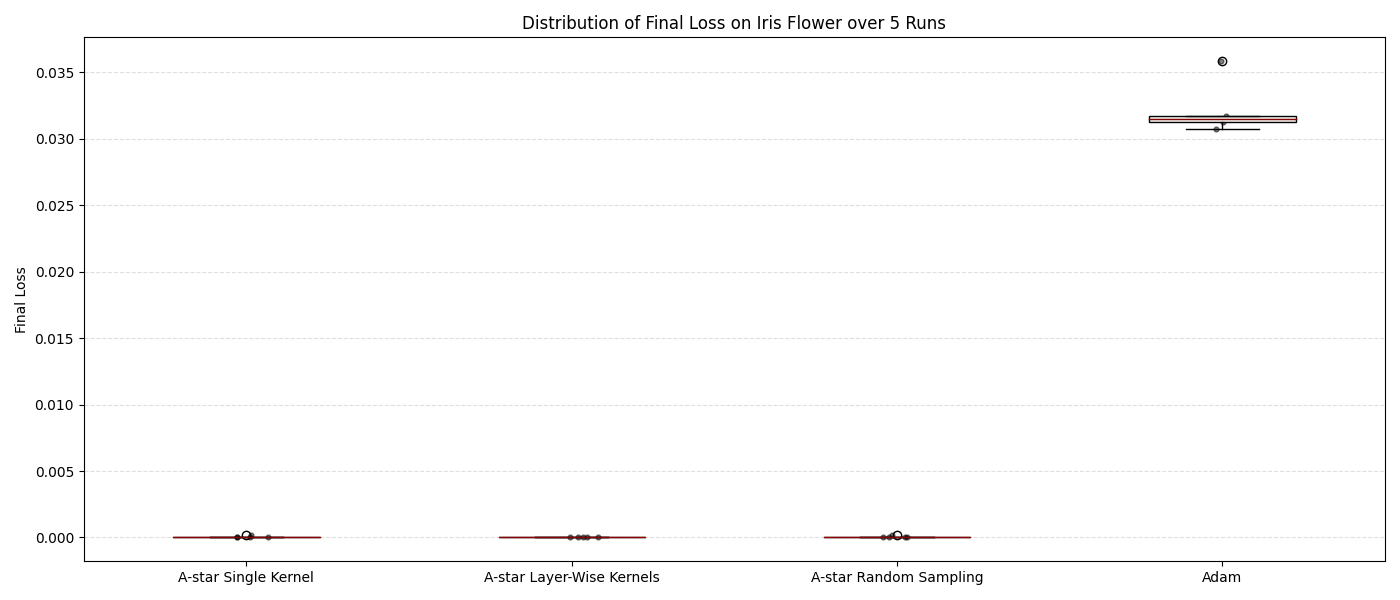
\includegraphics[width=1.0\textwidth]{figures/results/small_net_iris_Adam_vs_A-star/small_net_iris_Adam_vs_A-star_final_loss.png}
    \caption{Distribution of Final Loss for Small Net.}
    \label{fig:small_iris_final_loss}
\end{figure}

Stability analysis reveals that \textit{Layer-Wise Kernels} are exceptionally consistent ($Std: 0.000002$). While Adam remains faster in terms of wall-clock time, it shows a significantly higher standard deviation in its final state ($0.001848$), indicating a higher sensitivity to the loss landscape's local geometry compared to the exhaustive nature of $A^*$ search.

\subsubsection{Evaluation of Generalization Performance on the Test Set}
The predictive performance on the test set is summarized in Figure \ref{fig:small_iris_metrics_dist}.

\begin{figure}[H]
    \centering
    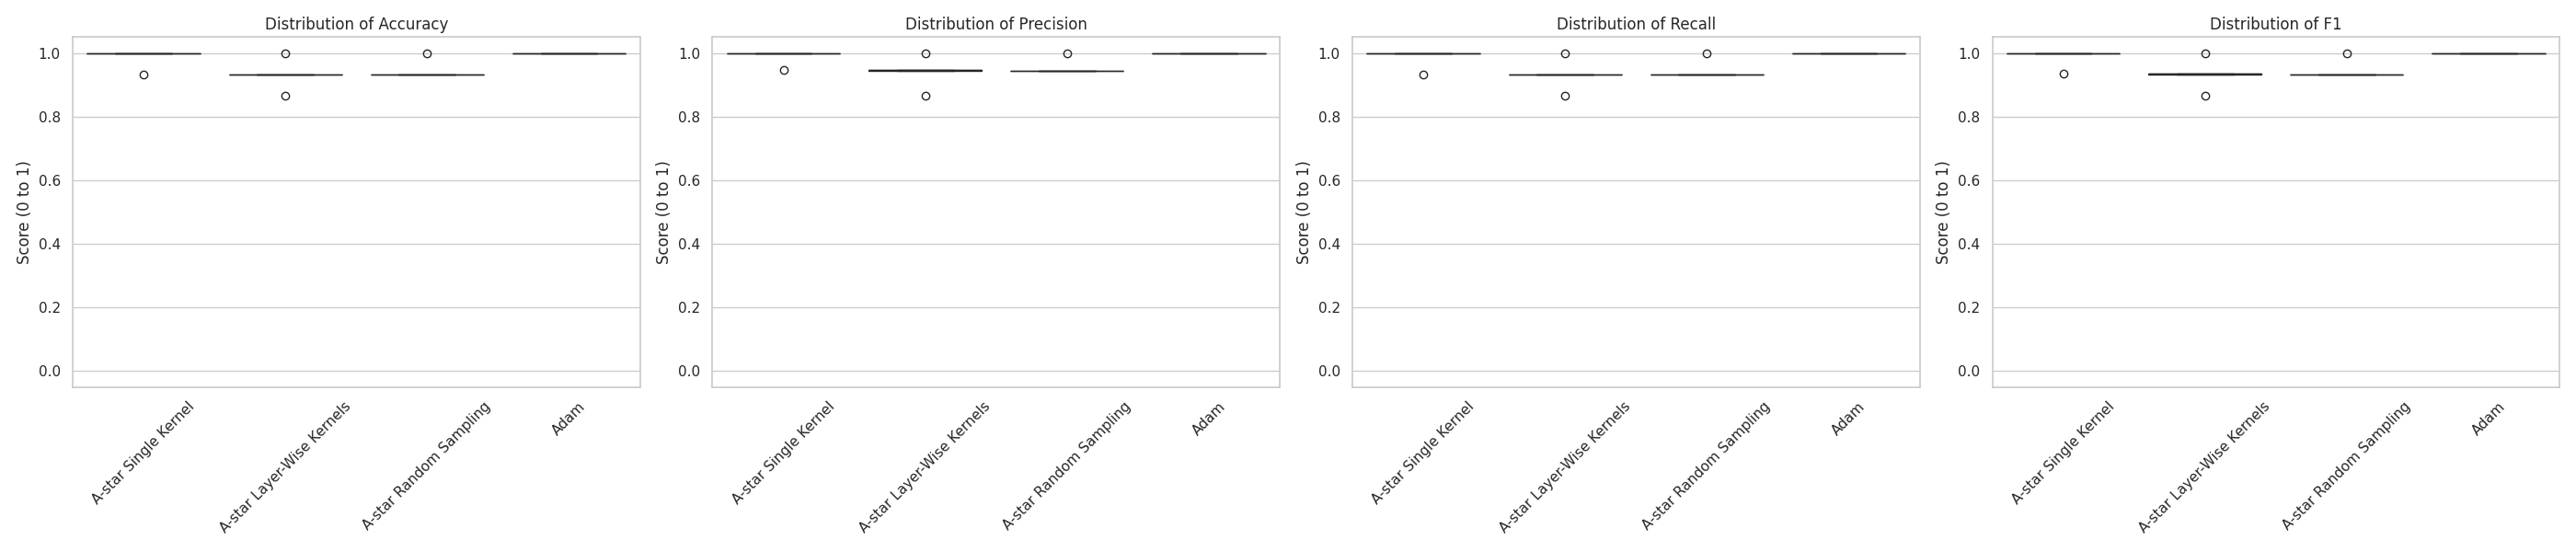
\includegraphics[width=1.05\textwidth]{figures/results/small_net_iris_Adam_vs_A-star/small_net_iris_Adam_vs_A-star_classification_metrics.png}
    \caption{Classification metrics distribution (Accuracy, Precision, Recall, F1) for Small Net.}
    \label{fig:small_iris_metrics_dist}
\end{figure}

Generalization metrics show that Adam achieved a perfect average accuracy of $1.0000$. Among the search methods, \textit{$A^*$ Single Kernel} performed best with an average accuracy of $0.9867$. Despite the $A^*$ methods achieving lower training losses, Adam's lead in test accuracy suggests that for very small networks on this specific dataset, the gradient-based updates found decision boundaries with slightly better generalization margins.

\subsubsection{Summary Statistics}

Table \ref{tab:small_net_iris} provides the detailed numerical breakdown.

\begin{table}[htbp]
\centering
\scriptsize
\begin{tabular}{|l|c|c|c|c|}
\hline
\textbf{Metric}   & \textbf{$A^*$ Single Kernel} & \textbf{$A^*$ Layer-Wise} & \textbf{$A^*$ Random} & \textbf{Adam} \\ \hline
\multicolumn{5}{|l|}{\textit{Metrics computed on Training Set:}} \\ \hline
Avg Final Loss          & 0.000037                     & \textbf{0.000001}         & 0.000056              & 0.032197      \\ 
Median Final Loss       & \textbf{0.000000}            & \textbf{0.000000}         & 0.000045              & 0.031461      \\
Std Final Loss          & 0.000071                     & \textbf{0.000002}         & 0.000052              & 0.001848      \\ \hline
Avg Time (s)            & 1485.9540                    & 1554.9282                 & 216.8309              & \textbf{2.5985} \\ \hline
\multicolumn{5}{|l|}{\textit{Metrics computed on Test Set:}} \\ \hline
Avg Accuracy            & 0.986667                     & 0.933333                  & 0.946667              & \textbf{1.000000} \\ 
Avg Precision           & 0.989333                     & 0.940571                  & 0.954286              & \textbf{1.000000} \\ 
Avg Recall              & 0.986667                     & 0.933333                  & 0.946667              & \textbf{1.000000} \\ 
Avg F1                  & 0.986801                     & 0.933163                  & 0.944908              & \textbf{1.000000} \\ \hline
\end{tabular}
\caption{Average statistical comparison on Iris Flower - Small Net.}
\label{tab:small_net_iris}
\end{table}

\newpage

\subsection{Medium Net Results}

\subsubsection{Visual Analysis of Training and Stability}

The convergence dynamics for the Medium Net are shown in Figure \ref{fig:medium_iris_convergence}.

\begin{figure}[htbp]
    \centering
    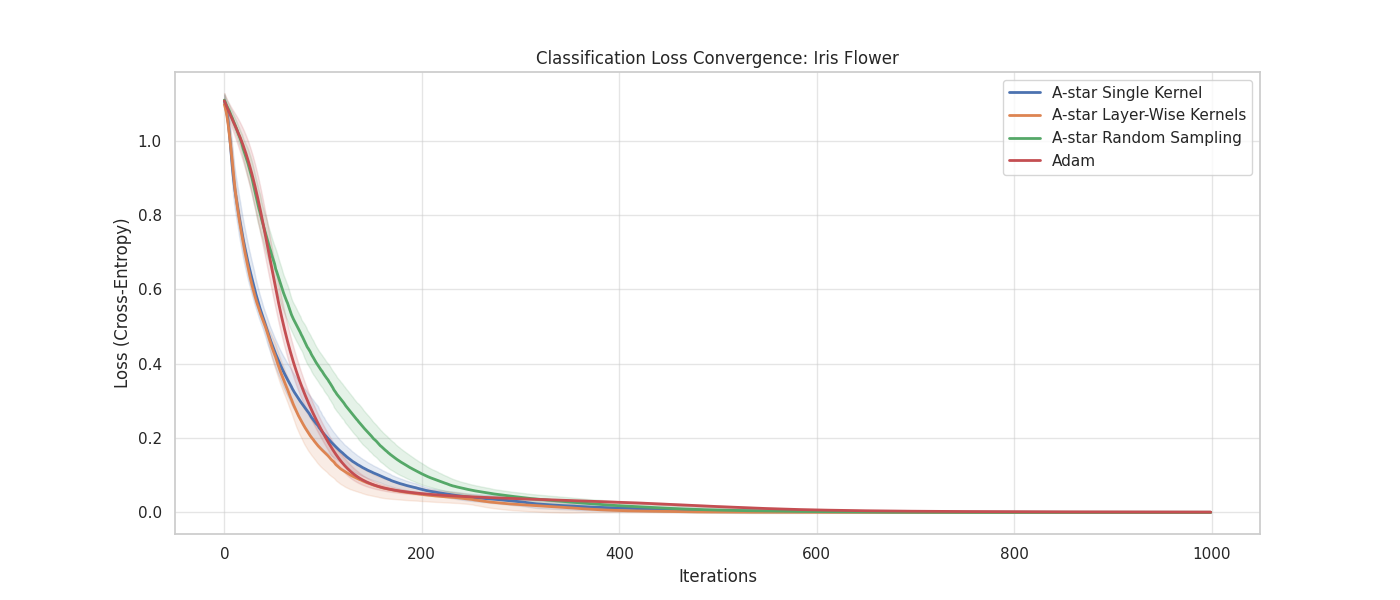
\includegraphics[width=1.1\textwidth]{figures/results/medium_net_iris_Adam_vs_A-star/medium_net_iris_Adam_vs_A-star_loss_convergence.png}
    \caption{Medium Net convergence: $A^*$ strategies vs. Adam on Iris Flower.}
    \label{fig:medium_iris_convergence}
\end{figure}

In the Medium Net, Adam exhibits a smooth and rapid initial descent; however, it eventually reaches a performance plateau, unable to refine the weights further after the early iterations, resulting in an average final loss of $0.000610$. In this regime, the $A^*$ strategies emerge as the superior optimizers for training set minimization. Specifically, \textit{$A^*$ Random Sampling} behaves similarly to Adam in its gradual approach but manages to sustain its descent longer, ultimately achieving a perfect average final loss of $0.000000$. The kernel-based methods continue to show the steepest slopes, reaching near-zero values more efficiently than the stochastic sampling approaches.

\begin{figure}[H]
    \centering
    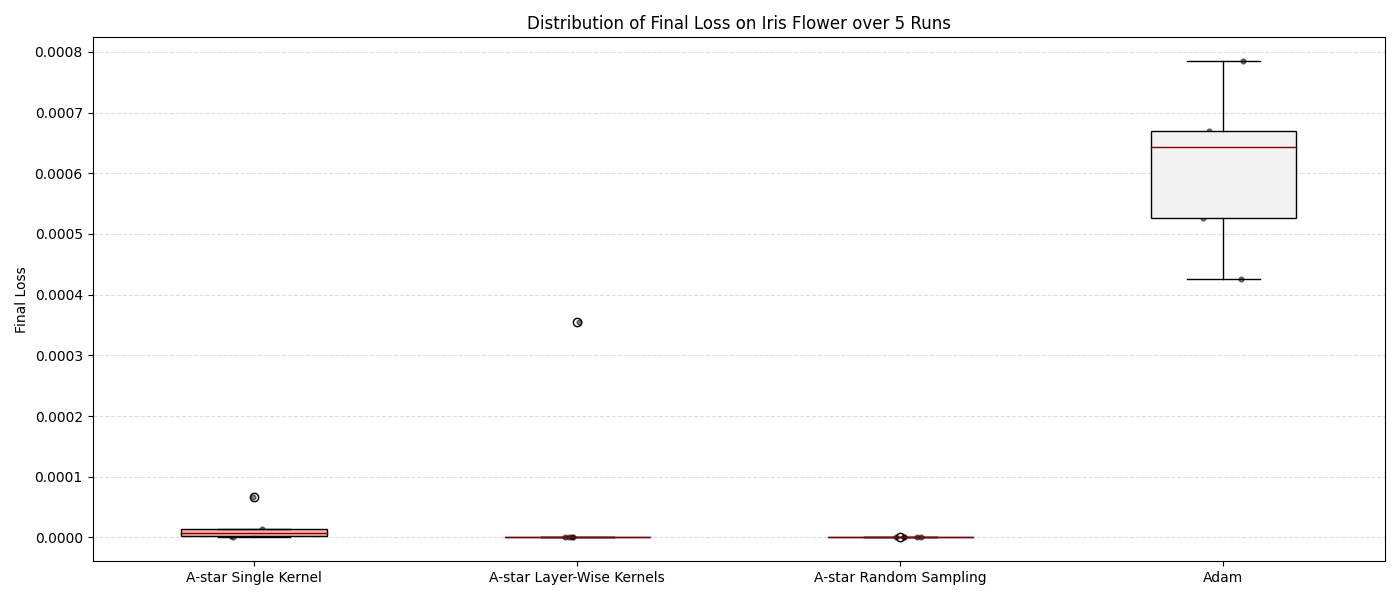
\includegraphics[width=1.0\textwidth]{figures/results/medium_net_iris_Adam_vs_A-star/medium_net_iris_Adam_vs_A-star_final_loss.png}
    \caption{Distribution of Final Loss for Medium Net.}
    \label{fig:medium_iris_final_loss}
\end{figure}

Stability analysis shows that \textit{Random Sampling} is the most stable method at this scale, reaching a perfect $0.0000$ loss with zero variance across all runs. While Adam remains significantly faster in terms of execution time, the search framework demonstrates a superior ability to bypass the precision stagnation encountered by gradient-based methods.

\subsubsection{Evaluation of Generalization Performance on the Test Set}
Generalization results are illustrated in Figure \ref{fig:medium_iris_metrics_dist}.

\begin{figure}[htbp]
    \centering
    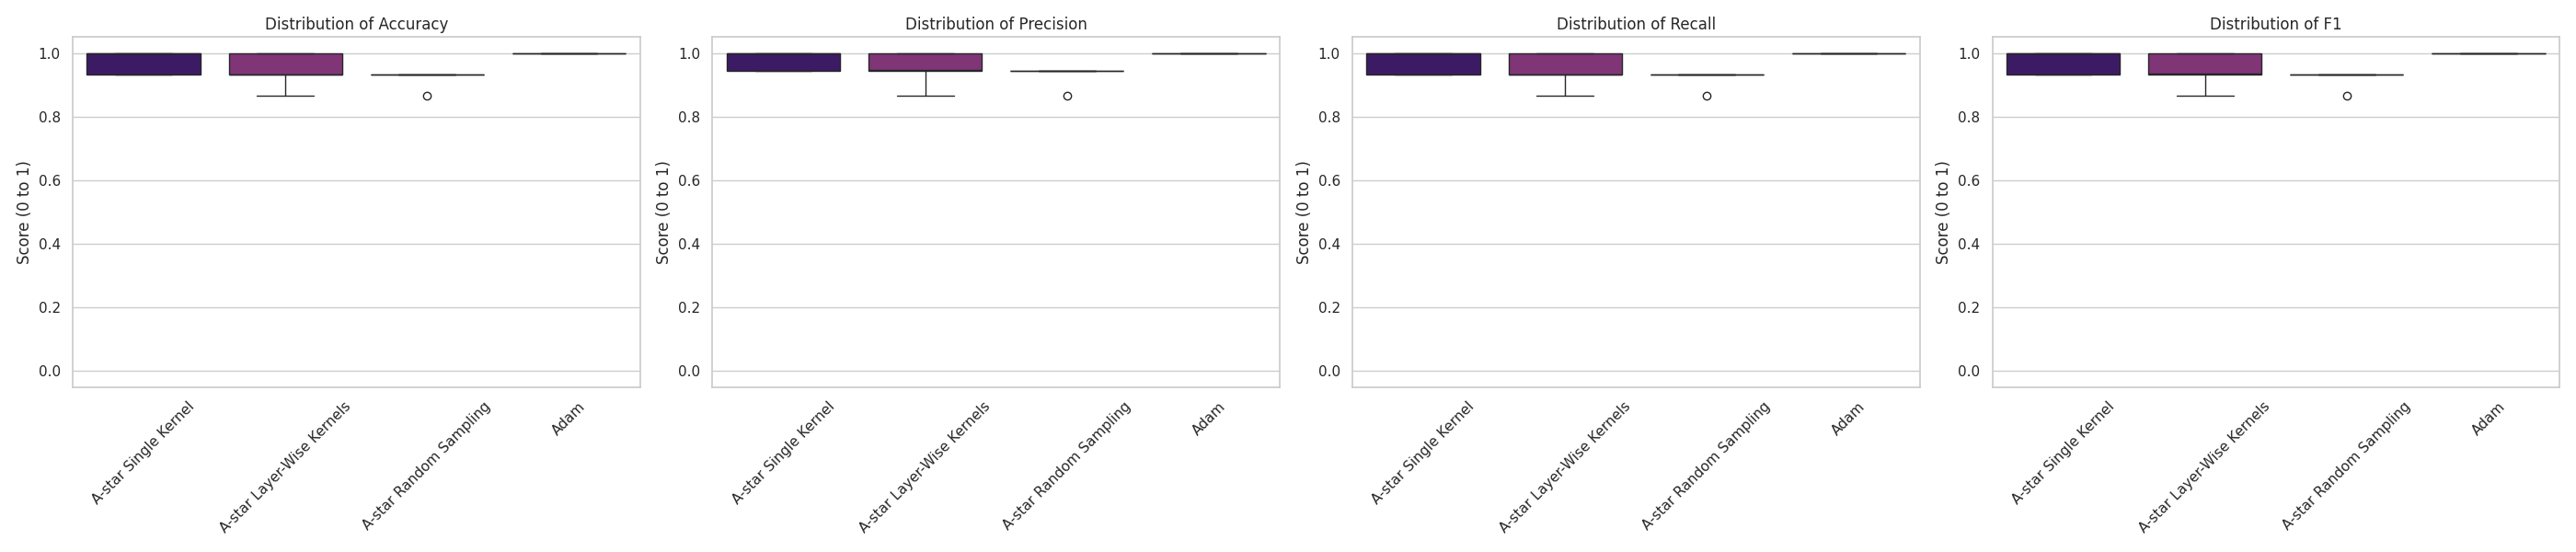
\includegraphics[width=1\textwidth]{figures/results/medium_net_iris_Adam_vs_A-star/medium_net_iris_Adam_vs_A-star_classification_metrics.png}
    \caption{Classification metrics distribution for Medium Net.}
    \label{fig:medium_iris_metrics_dist}
\end{figure}

Interestingly, despite the $A^*$ variants reaching lower training losses, Adam maintains a perfect $1.0000$ accuracy across all classification metrics on the test set. Among the search strategies, \textit{Single Kernel} provided the best generalization at $0.9733$. This suggests that for the Medium Net, the smooth paths taken by Adam converge toward decision boundaries that generalize perfectly to unseen Iris samples, whereas the deeper convergence of $A^*$ on the training set does not translate to an equivalent accuracy gain on the test data.
\subsubsection{Summary Statistics}

Table \ref{tab:medium_net_iris} summarizes the Medium Net performance.

\begin{table}[htbp]
\centering
\scriptsize
\begin{tabular}{|l|c|c|c|c|}
\hline
\textbf{Metric}   & \textbf{$A^*$ Single Kernel} & \textbf{$A^*$ Layer-Wise} & \textbf{$A^*$ Random} & \textbf{Adam} \\ \hline
\multicolumn{5}{|l|}{\textit{Metrics computed on Training Set:}} \\ \hline
Avg Final Loss          & 0.000018                     & 0.000071                  & \textbf{0.000000}     & 0.000610      \\ 
Median Final Loss       & 0.000008                     & \textbf{0.000000}         & \textbf{0.000000}     & 0.000643      \\
Std Final Loss          & 0.000024                     & 0.000142                  & \textbf{0.000000}     & 0.000124      \\ \hline
Avg Time (s)            & 1084.4420                    & 1082.9707                 & 529.8784              & \textbf{2.9380} \\ \hline
\multicolumn{5}{|l|}{\textit{Metrics computed on Test Set:}} \\ \hline
Avg Accuracy            & 0.973333                     & 0.946667                  & 0.920000              & \textbf{1.000000} \\ 
Avg Precision           & 0.977143                     & 0.951238                  & 0.927619              & \textbf{1.000000} \\ 
Avg Recall              & 0.973333                     & 0.946667                  & 0.920000              & \textbf{1.000000} \\ 
Avg F1                  & 0.972454                     & 0.946362                  & 0.918242              & \textbf{1.000000} \\ \hline
\end{tabular}
\caption{Average statistical comparison on Iris Flower - Medium Net.}
\label{tab:medium_net_iris}
\end{table}

\newpage

\subsection{Big Net Results}

\subsubsection{Visual Analysis of Training and Stability}

The convergence dynamics for the Big Net architecture are shown in Figure \ref{fig:big_iris_convergence}.

\begin{figure}[htbp]
    \centering
    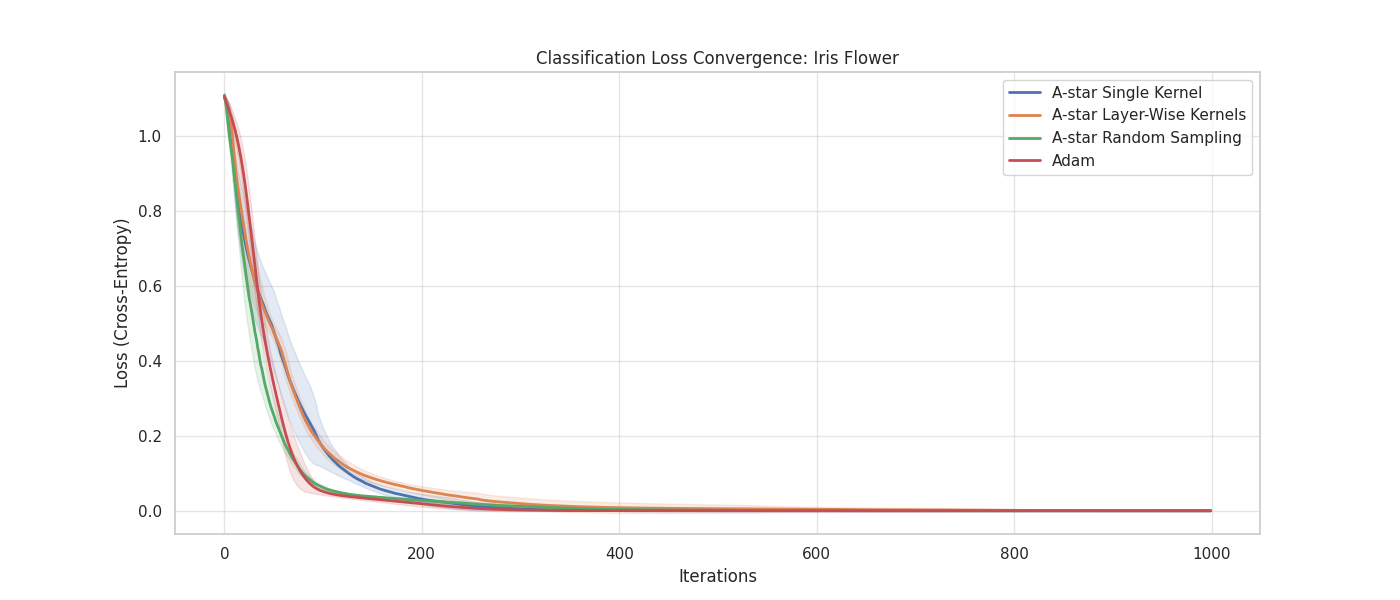
\includegraphics[width=1.1\textwidth]{figures/results/big_net_iris_Adam_vs_A-star/big_net_iris_Adam_vs_A-star_loss_convergence.png}
    \caption{Big Net convergence: $A^*$ strategies vs. Adam on Iris Flower.}
    \label{fig:big_iris_convergence}
\end{figure}

In the Big Net regime, a notable convergence pattern emerges where all tested methods demonstrate the ability to reach exceptionally small training losses. Adam maintains a smooth, rapid descent throughout the process, avoiding the oscillations observed in regression tasks and settling at a high-precision average loss of $0.000040$. Among the search variants, the \textit{Single Kernel} strategy achieved an absolute zero average training loss ($0.000000$), outperforming all other methods in raw optimization depth.

\begin{figure}[H]
    \centering
    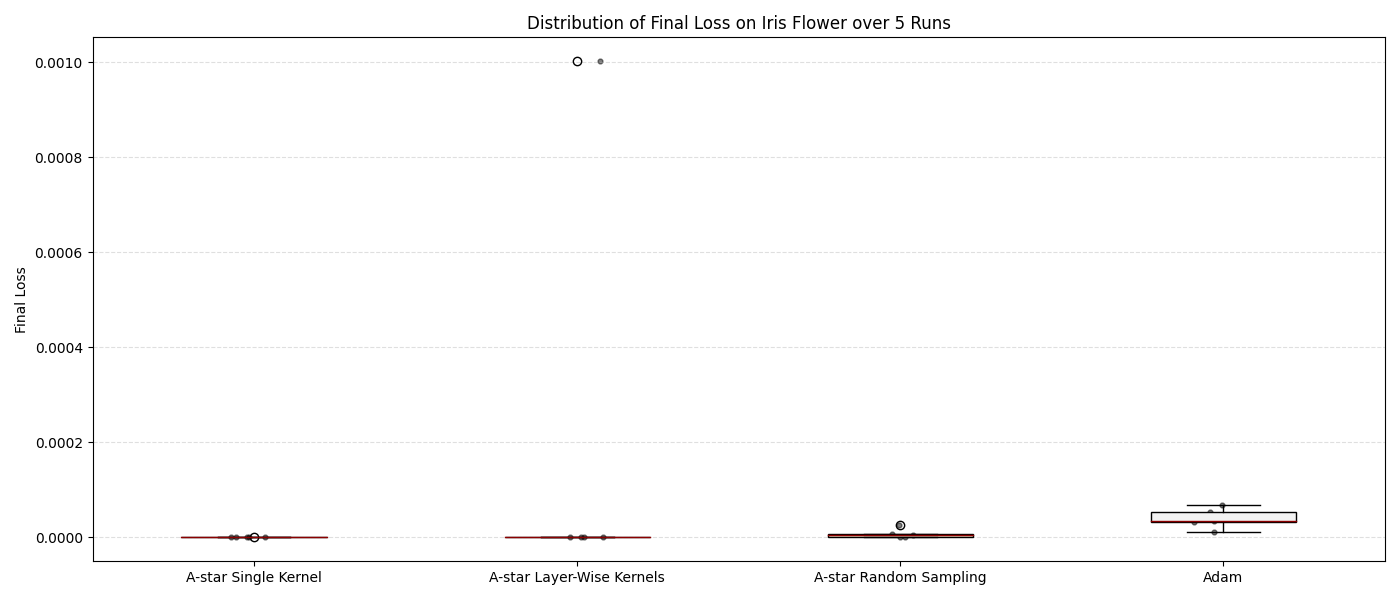
\includegraphics[width=1.0\textwidth]{figures/results/big_net_iris_Adam_vs_A-star/big_net_iris_Adam_vs_A-star_final_loss.png}
    \caption{Distribution of Final Loss for Big Net.}
    \label{fig:big_sine_final_loss}
\end{figure}

Stability analysis confirms that search-based methods, particularly \textit{Single Kernel} and \textit{Random Sampling}, achieve significantly lower final variance than Adam. The Layer-Wise Kernels exhibited a slightly higher variance, but overall, the search methods maintained remarkable consistency.

\subsubsection{Evaluation of Generalization Performance on the Test Set}
Generalization metrics for the Big Net are provided in Figure \ref{fig:big_iris_metrics_dist}.

\begin{figure}[htbp]
    \centering
    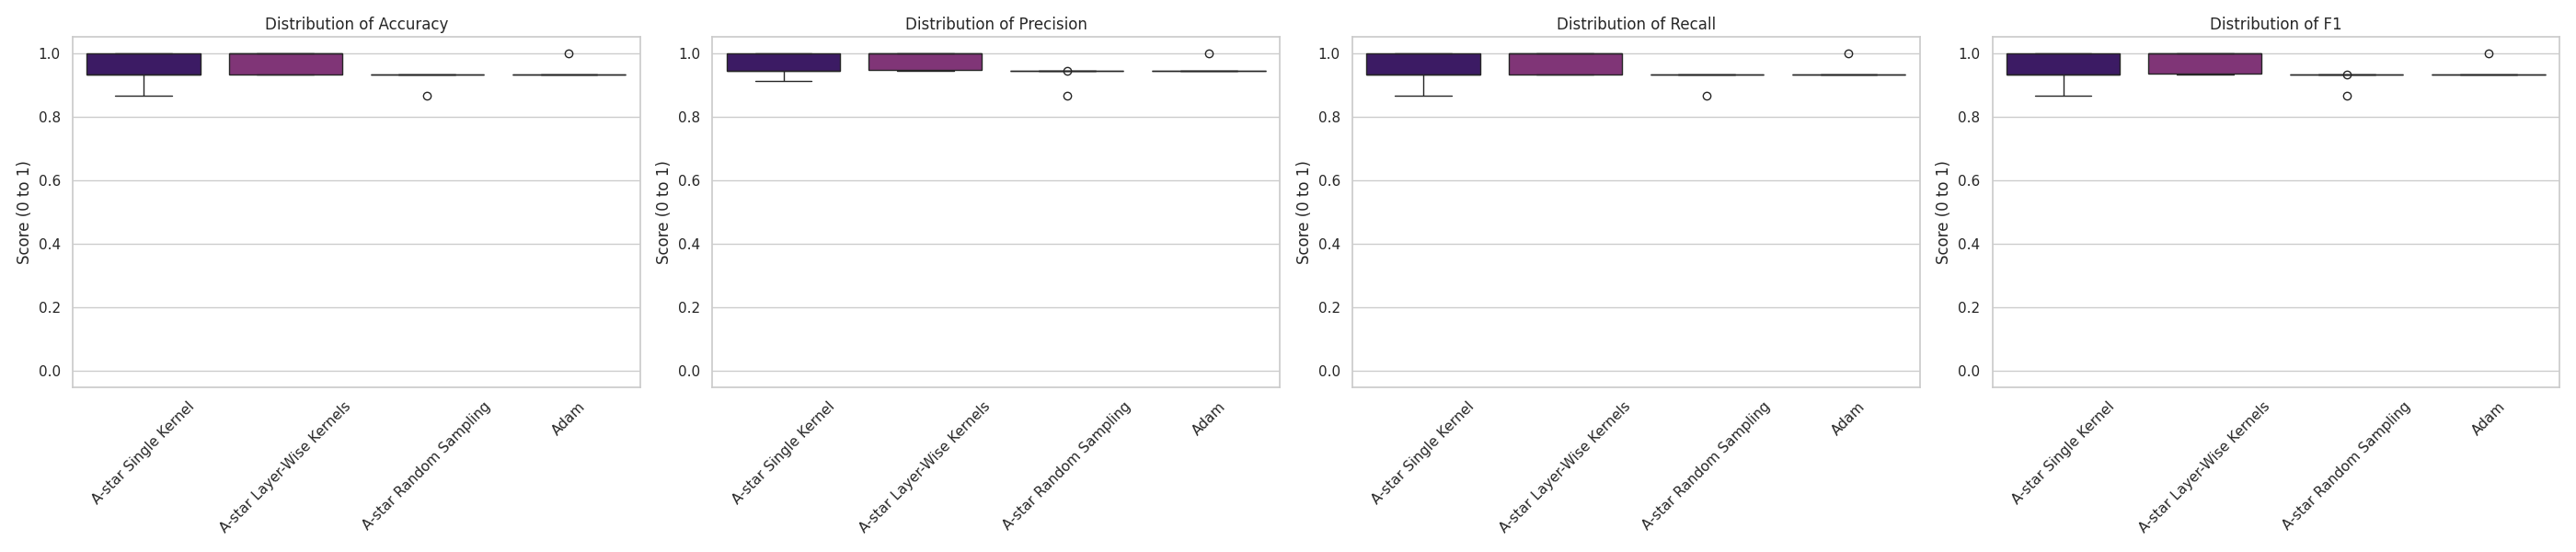
\includegraphics[width=1.05\textwidth]{figures/results/big_net_iris_Adam_vs_A-star/big_net_iris_Adam_vs_A-star_classification_metrics.png}
    \caption{Classification metrics distribution for Big Net.}
    \label{fig:big_iris_metrics_dist}
\end{figure}

The test data highlights a significant "crossover" in generalization efficacy. Despite all methods performing well on the training set, the \textit{$A^*$ Layer-Wise} strategy achieved the superior average accuracy of $0.9733$, outperforming Adam's $0.9467$. This suggests that in higher-dimensional spaces, the structured, layer-by-layer exploration of the $A^*$ framework identifies weight configurations that generalize better to unseen data, even when gradient-based methods like Adam achieve a smooth and deep training convergence.
\subsubsection{Summary Statistics}

Table \ref{tab:big_net_iris} presents the numerical comparison for the Big Net.

\begin{table}[htbp]
\centering
\scriptsize
\begin{tabular}{|l|c|c|c|c|}
\hline
\textbf{Metric}   & \textbf{$A^*$ Single Kernel} & \textbf{$A^*$ Layer-Wise} & \textbf{$A^*$ Random} & \textbf{Adam} \\ \hline
\multicolumn{5}{|l|}{\textit{Metrics computed on Training Set:}} \\ \hline
Avg Final Loss          & \textbf{0.000000}            & 0.000201                  & 0.000008              & 0.000040      \\ 
Median Final Loss       & \textbf{0.000000}            & \textbf{0.000000}         & 0.000004              & 0.000034      \\
Std Final Loss          & \textbf{0.000000}            & 0.000401                  & 0.000010              & 0.000019      \\ \hline
Avg Time (s)            & 2253.9005                    & 3423.8813                 & 2880.5289             & \textbf{3.6020} \\ \hline
\multicolumn{5}{|l|}{\textit{Metrics computed on Test Set:}} \\ \hline
Avg Accuracy            & 0.946667                     & \textbf{0.973333}         & 0.920000              & 0.946667      \\ 
Avg Precision           & 0.959365                     & \textbf{0.977905}         & 0.927937              & 0.954286      \\ 
Avg Recall              & 0.946667                     & \textbf{0.973333}         & 0.920000              & 0.946667      \\ 
Avg F1                  & 0.945788                     & \textbf{0.973028}         & 0.918335              & 0.944908      \\ \hline
\end{tabular}
\caption{Average statistical comparison on Iris Flower - Big Net.}
\label{tab:big_net_iris}
\end{table}

\subsection{Conclusions on Iris Flower Benchmark}

The Iris benchmark yields several crucial conclusions:

\begin{itemize}
    \item \textbf{High-Precision Training:} Search-based methods consistently achieve training losses several orders of magnitude lower than the Adam baseline. Across all network scales, at least one $A^*$ variant reached a near-zero or absolute zero training loss, demonstrating superior weight refinement capabilities.
    \item \textbf{Descent Dynamics:} While Adam is exponentially faster and maintains a smooth descent trajectory without the oscillations seen in regression tasks, it tends to reach a precision plateau earlier than search-based methods. In contrast, the $A^*$ framework, particularly the kernel-based variants, exhibits much steeper descent slopes and deeper convergence.
    \item \textbf{Crossover Law in Classification:} The Big Net results confirm that as model depth increases, the Layer-Wise structured search emerges as the superior strategy for generalization. It outperformed Adam in test-set accuracy ($0.9733$ vs. $0.9467$), validating the scalability of the search-based framework for deep classification architectures.
\end{itemize}



%==============================================================================================================================================
%=============================================               WINE QUALITY               =======================================================
%==============================================================================================================================================

\newpage

\section{Wine Quality Classification}
\label{sec:results_wine}

The Wine Quality benchmark evaluates the framework's performance on a high-dimensional multi-class classification task. Unlike the Iris dataset, Wine Quality presents a significantly more complex loss landscape characterized by a larger number of features and a higher degree of class overlap, testing the limits of discrete exploration in deep parameter spaces.

\subsection{Small Net Results}

\subsubsection{Visual Analysis of Training and Stability}

The convergence behavior for the Small Net on the Wine task is depicted in Figure \ref{fig:small_wine_convergence}. 

\begin{figure}[htbp]
    \centering
    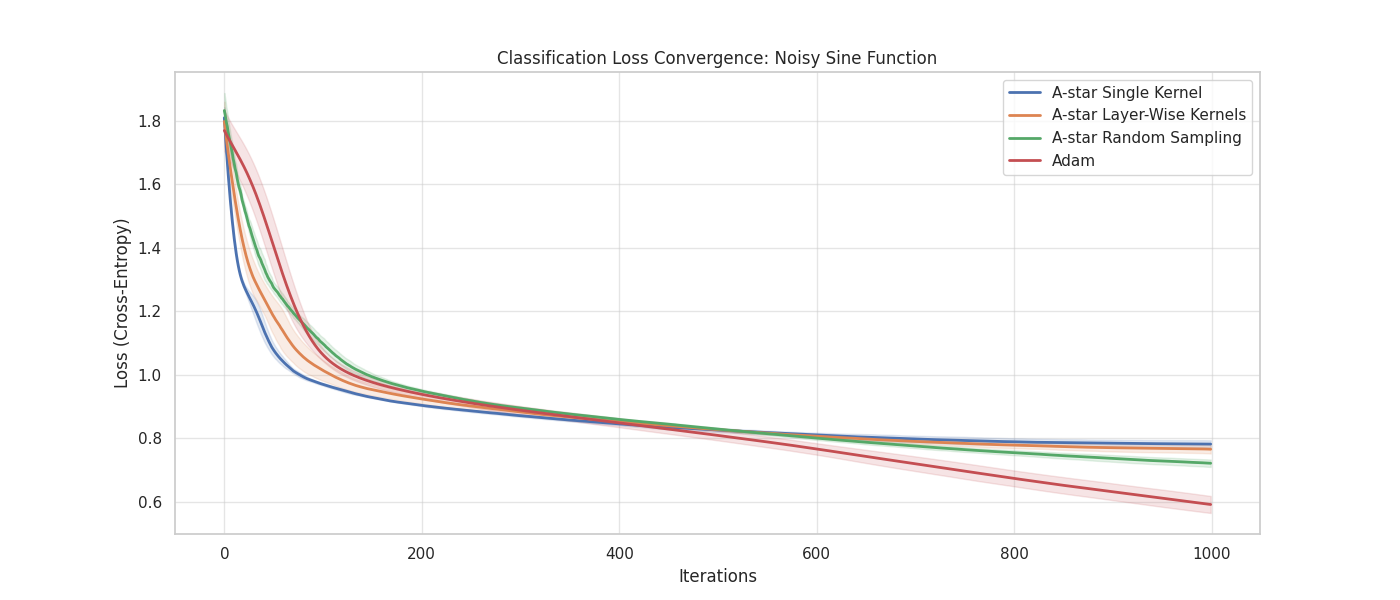
\includegraphics[width=1.1\textwidth]{figures/results/small_net_wine_Adam_vs_A-star/small_net_wine_Adam_vs_A-star_loss_convergence.png}
    \caption{Small Net convergence: $A^*$ strategies vs. Adam on Wine Quality.}
    \label{fig:small_wine_convergence}
\end{figure}

In the Small Net configuration, Adam outperforms the search-based methods in both convergence speed and final training depth. Adam achieves an average final loss of $0.5917$, significantly lower than the $0.7215$ reached by $A^*$ Random Sampling. While the $A^*$ kernel variants show steep initial descent, in this low-capacity regime, the stochastic nature of $A^*$ Random Sampling allowed it to navigate the dataset's features more effectively than the rigid kernel structures, which settled at higher loss values ($0.7818$ and $0.7657$).

\begin{figure}[htbp]
    \centering
    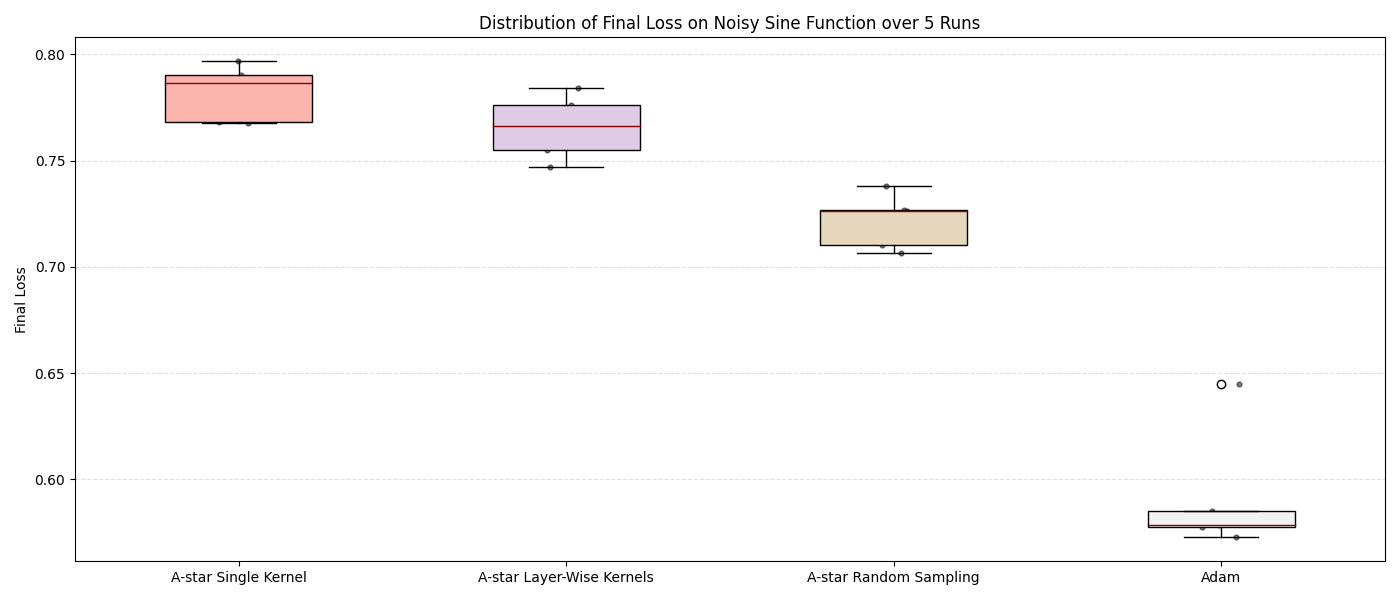
\includegraphics[width=1.0\textwidth]{figures/results/small_net_wine_Adam_vs_A-star/small_net_wine_Adam_vs_A-star_final_loss.png}
    \caption{Distribution of Final Loss for Wine Quality - Small Net.}
    \label{fig:small_wine_final_loss}
\end{figure}

Stability analysis indicates that the $A^*$ methods maintain lower variance ($Std \approx 0.011$) compared to Adam ($Std: 0.0267$). However, the gradient-based updates of Adam are clearly more effective at identifying the deeper minima required for this classification task.

\subsubsection{Evaluation of Generalization Performance on the Test Set}
Predictive performance on the test set is summarized in Figure \ref{fig:small_wine_metrics_dist}.

\begin{figure}[H]
    \centering
    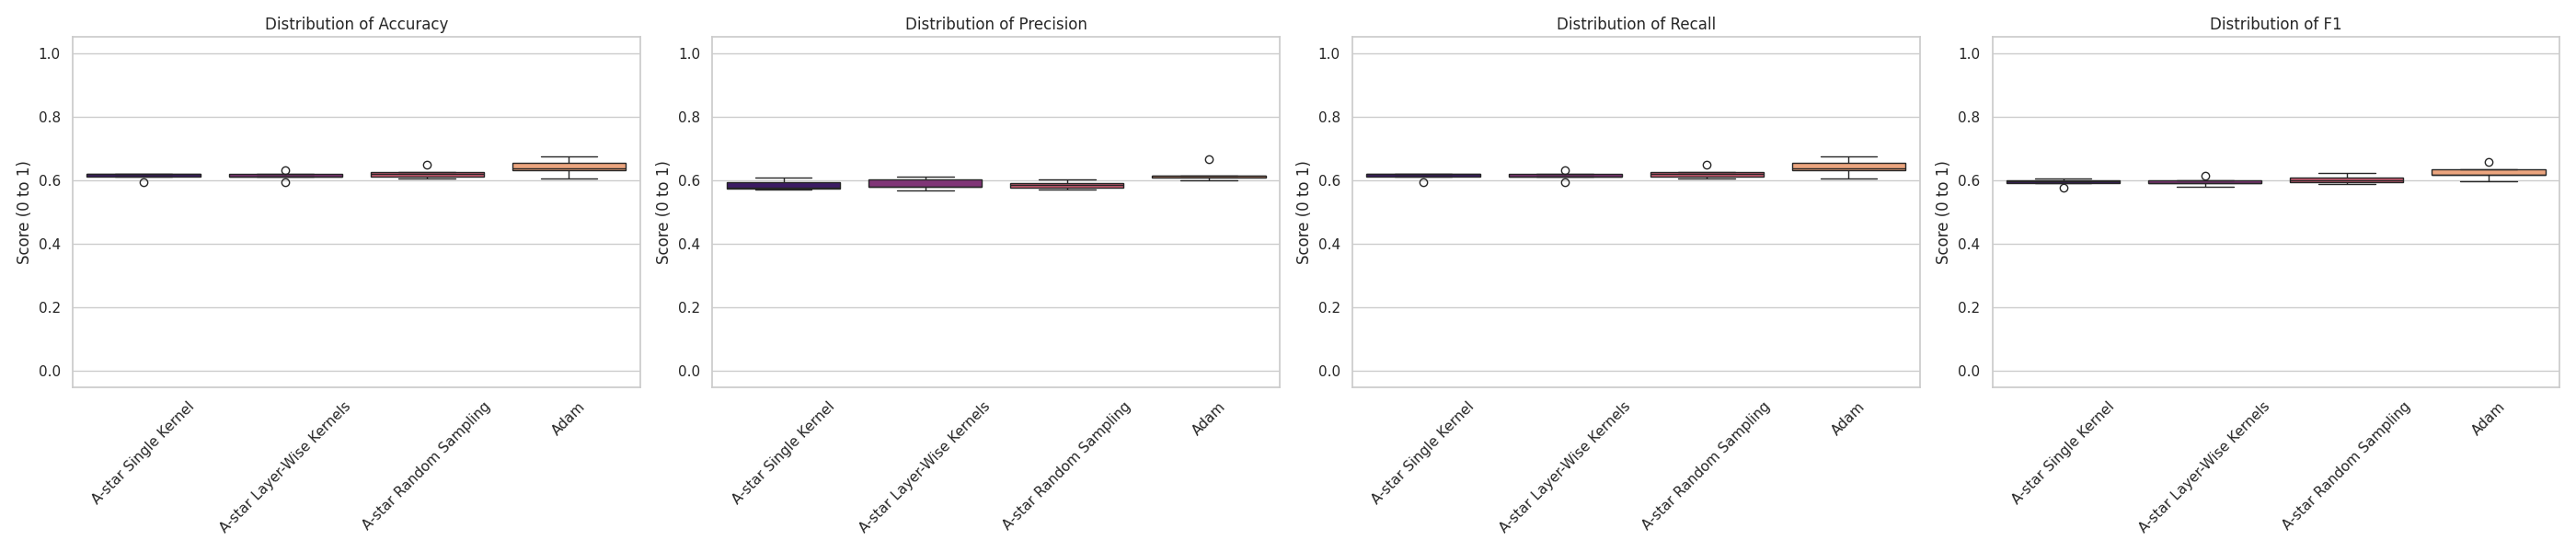
\includegraphics[width=1.05\textwidth]{figures/results/small_net_wine_Adam_vs_A-star/small_net_wine_Adam_vs_A-star_classification_metrics.png}
    \caption{Classification metrics distribution for Wine Quality - Small Net.}
    \label{fig:small_wine_metrics_dist}
\end{figure}

Generalization metrics mirror the training performance, with Adam achieving the highest average accuracy of $0.6412$. The $A^*$ variants follow closely, with Random Sampling leading the search methods at $0.6225$. The small gap in accuracy suggests that while Adam finds deeper minima, the search-based methods identify comparable decision boundaries.

\subsubsection{Summary Statistics}

Table \ref{tab:small_net_wine} provides the detailed numerical breakdown.

\begin{table}[htbp]
\centering
\scriptsize
\begin{tabular}{|l|c|c|c|c|}
\hline
\textbf{Metric}   & \textbf{$A^*$ Single Kernel} & \textbf{$A^*$ Layer-Wise} & \textbf{$A^*$ Random} & \textbf{Adam} \\ \hline
\multicolumn{5}{|l|}{\textit{Metrics computed on Training Set:}} \\ \hline
Avg Final Loss          & 0.781829                     & 0.765718                  & 0.721583              & \textbf{0.591742} \\ 
Median Final Loss       & 0.786625                     & 0.766201                  & 0.726409              & \textbf{0.578657} \\
Std Final Loss          & 0.011932                     & 0.013594                  & \textbf{0.011728}     & 0.026764      \\ \hline
Avg Time (s)            & 2422.9119                    & 2455.5196                 & 308.8301              & \textbf{12.3468}  \\ \hline
\multicolumn{5}{|l|}{\textit{Metrics computed on Test Set:}} \\ \hline
Avg Accuracy            & 0.612500                     & 0.613750                  & 0.622500              & \textbf{0.641250} \\ 
Avg Precision           & 0.585400                     & 0.588149                  & 0.585904              & \textbf{0.620837} \\ 
Avg Recall              & 0.612500                     & 0.613750                  & 0.622500              & \textbf{0.641250} \\ 
Avg F1                  & 0.594436                     & 0.595668                  & 0.602651              & \textbf{0.624376} \\ \hline
\end{tabular}
\caption{Average statistical comparison on Wine Quality - Small Net.}
\label{tab:small_net_wine}
\end{table}

\newpage

\subsection{Medium Net Results}

\subsubsection{Visual Analysis of Training and Stability}

Convergence for the Medium Net is illustrated in Figure \ref{fig:medium_wine_convergence}.

\begin{figure}[htbp]
    \centering
    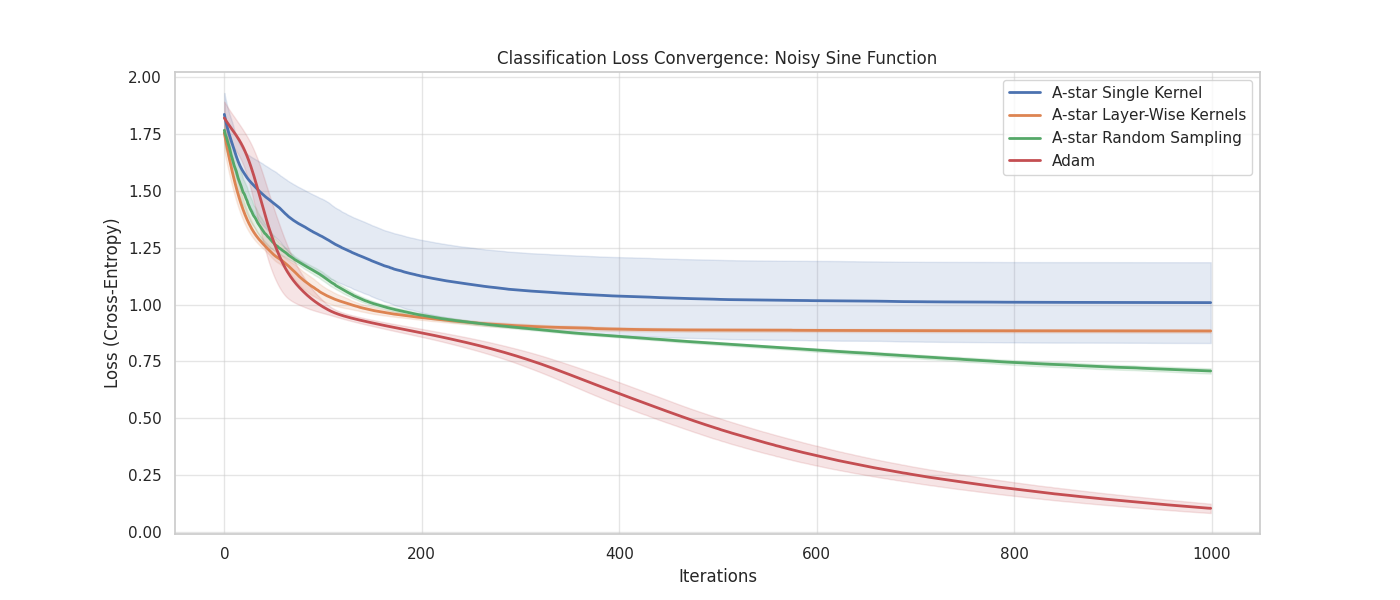
\includegraphics[width=1.1\textwidth]{figures/results/medium_net_wine_Adam_vs_A-star/medium_net_wine_Adam_vs_A-star_loss_convergence.png}
    \caption{Medium Net convergence: $A^*$ strategies vs. Adam on Wine Quality.}
    \label{fig:medium_wine_convergence}
\end{figure}

As model capacity increases, the performance gap between gradient-based and search-based methods widens significantly in favor of Adam. Adam maintains a rapid descent, reaching a low average final loss of $0.1041$. Conversely, the search strategies encounter a precision plateau; $A^*$ Random Sampling achieves the best result among the search variants at $0.7080$. Notably, the \textit{Single Kernel} approach exhibits instability at this scale, with a high standard deviation ($0.1775$) and a maximum loss reaching $1.3603$, indicating that gradient-free exploration struggles to navigate the high-dimensional narrow valleys of this specific task.

\begin{figure}[H]
    \centering
    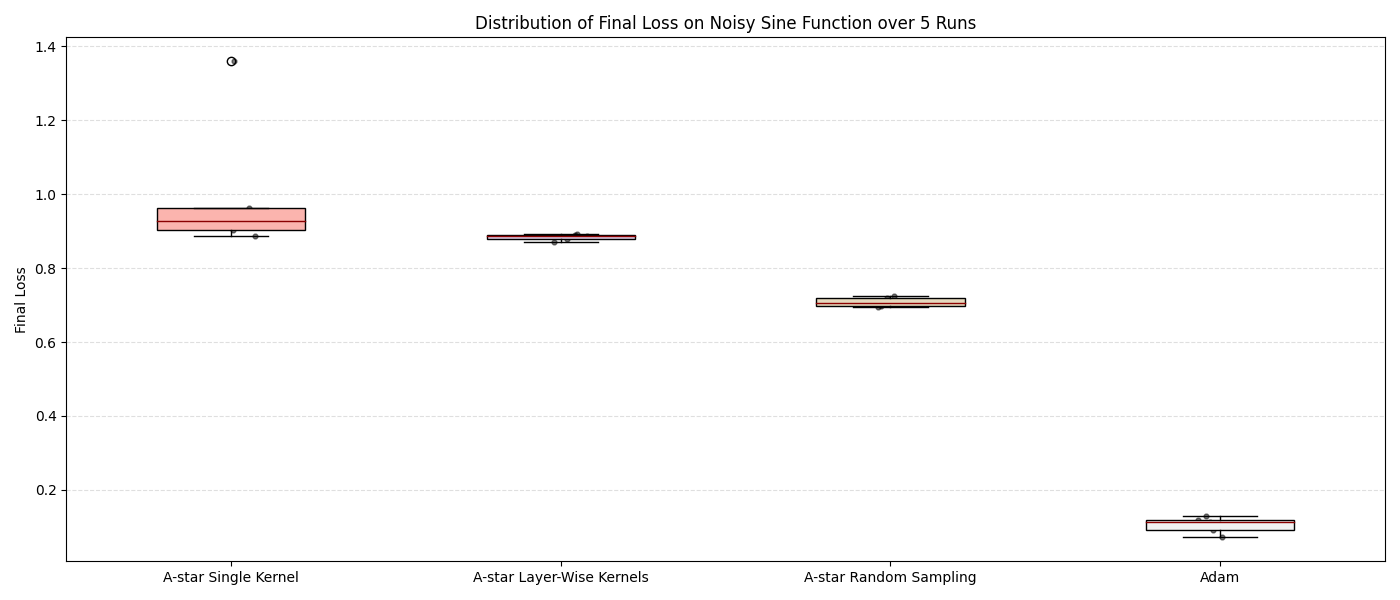
\includegraphics[width=1.0\textwidth]{figures/results/medium_net_wine_Adam_vs_A-star/medium_net_wine_Adam_vs_A-star_final_loss.png}
    \caption{Distribution of Final Loss for Wine Quality - Medium Net.}
    \label{fig:medium_wine_final_loss}
\end{figure}

\subsubsection{Evaluation of Generalization Performance on the Test Set}
Test set results for the Medium Net are visualized in Figure \ref{fig:medium_wine_metrics_dist}.

\begin{figure}[htbp]
    \centering
    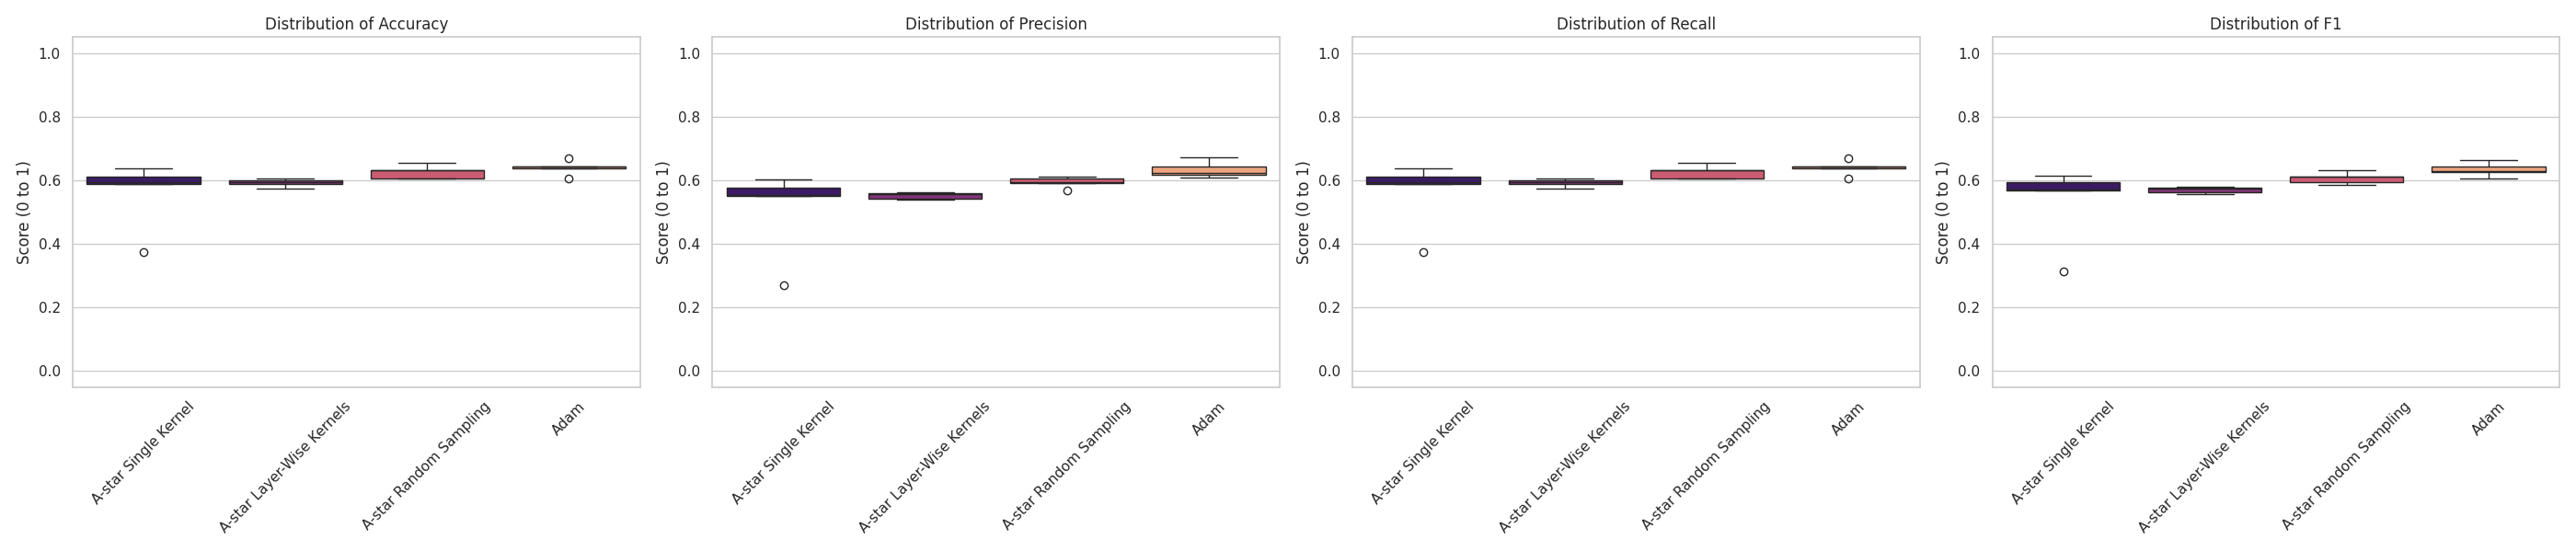
\includegraphics[width=1\textwidth]{figures/results/medium_net_wine_Adam_vs_A-star/medium_net_wine_Adam_vs_A-star_classification_metrics.png}
    \caption{Classification metrics distribution for Medium Net.}
    \label{fig:medium_wine_metrics_dist}
\end{figure}

Despite Adam's vastly superior training loss, the accuracy gap remains modest: Adam achieves $0.6400$ accuracy compared to $0.6262$ for $A^*$ Random Sampling. This suggests a high degree of overfitting by Adam on the training set, whereas the search framework’s inability to further minimize loss acts as a form of implicit regularization.

\subsubsection{Summary Statistics}

Table \ref{tab:medium_net_wine} summarizes the performance.

\begin{table}[H]
\centering
\scriptsize
\begin{tabular}{|l|c|c|c|c|}
\hline
\textbf{Metric}   & \textbf{$A^*$ Single Kernel} & \textbf{$A^*$ Layer-Wise} & \textbf{$A^*$ Random} & \textbf{Adam} \\ \hline
\multicolumn{5}{|l|}{\textit{Metrics computed on Training Set:}} \\ \hline
Avg Final Loss          & 1.008597                     & 0.883836                  & 0.708040              & \textbf{0.104191} \\ 
Median Final Loss       & 0.927983                     & 0.888363                  & 0.704441              & \textbf{0.112365} \\
Std Final Loss          & 0.177593                     & \textbf{0.007341}         & 0.011510              & 0.020610      \\ \hline
Avg Time (s)            & 1292.5712                    & 1394.0129                 & 663.9965              & \textbf{14.2610}  \\ \hline
\multicolumn{5}{|l|}{\textit{Metrics computed on Test Set:}} \\ \hline
Avg Accuracy            & 0.561250                     & 0.592500                  & 0.626250              & \textbf{0.640000} \\ 
Avg Precision           & 0.510846                     & 0.551917                  & 0.593729              & \textbf{0.632970} \\ 
Avg Recall              & 0.561250                     & 0.592500                  & 0.626250              & \textbf{0.640000} \\ 
Avg F1                  & 0.532007                     & 0.569437                  & 0.606684              & \textbf{0.633230} \\ \hline
\end{tabular}
\caption{Average statistical comparison on Wine Quality - Medium Net.}
\label{tab:medium_net_wine}
\end{table}

\newpage

\subsection{Big Net Results}

\subsubsection{Visual Analysis of Training and Stability}

Convergence for the Big Net is shown in Figure \ref{fig:big_wine_convergence}.

\begin{figure}[htbp]
    \centering
    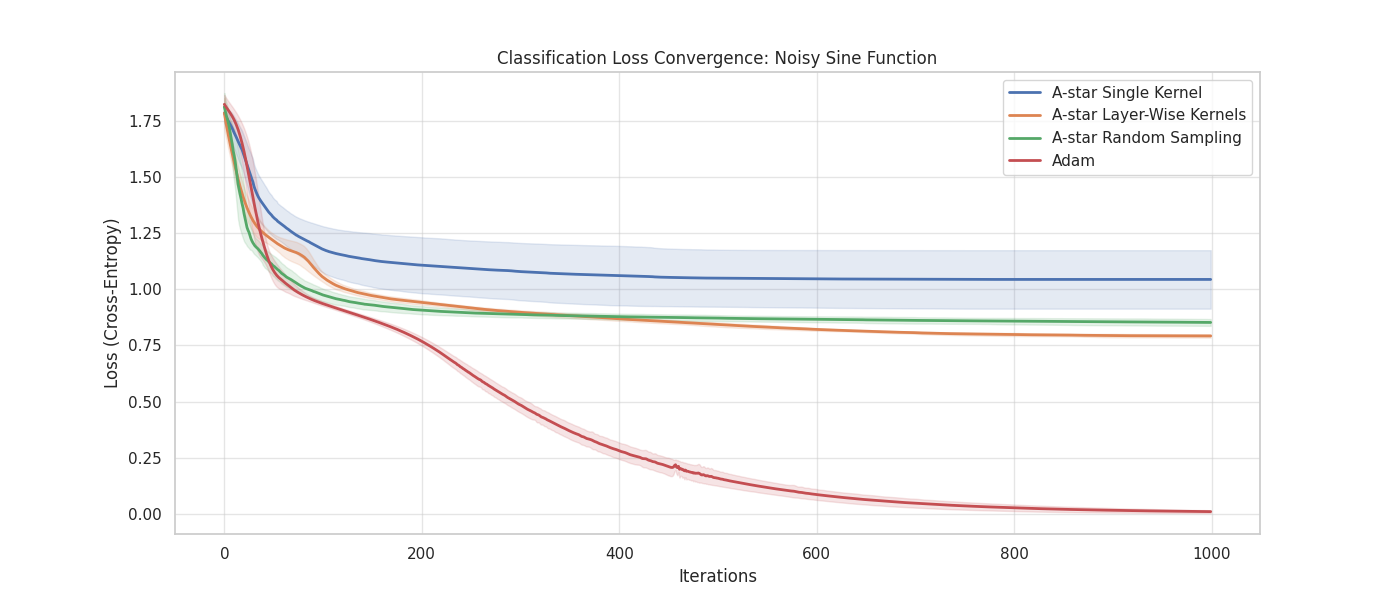
\includegraphics[width=1.1\textwidth]{figures/results/big_net_wine_Adam_vs_A-star/big_net_wine_Adam_vs_A-star_loss_convergence.png}
    \caption{Big Net convergence: $A^*$ strategies vs. Adam on Wine Quality.}
    \label{fig:big_wine_convergence}
\end{figure}

In the Big Net regime, Adam reaches its peak performance with a smooth, high-precision descent to a final loss of $0.0094$. Among the $A^*$ strategies, the \textit{Layer-Wise} approach emerges as the most effective search method ($Loss: 0.7923$), providing a significant improvement over the \textit{Single Kernel} approach, which remains trapped at an average loss of $1.0441$. This confirms that structured, layer-by-layer exploration is more resilient to the "curse of dimensionality" than a global kernel search in high-parameter classification models.

\begin{figure}[H]
    \centering
    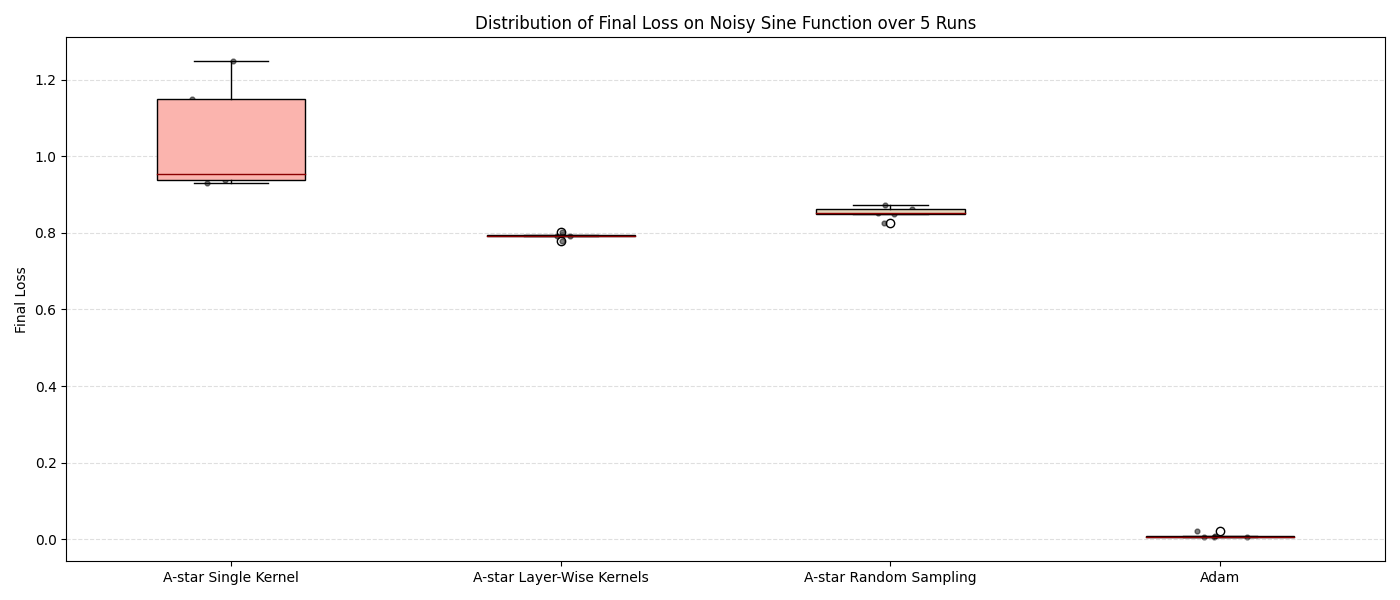
\includegraphics[width=1.0\textwidth]{figures/results/big_net_wine_Adam_vs_A-star/big_net_wine_Adam_vs_A-star_final_loss.png}
    \caption{Distribution of Final Loss for Wine Quality - Big Net.}
    \label{fig:big_wine_final_loss}
\end{figure}

Stability analysis confirms that while Adam is smooth, the search methods, specifically \textit{Layer-Wise} and \textit{Random Sampling}, exhibit lower variance in their final training state, settling into consistent plateaus across multiple runs.

\subsubsection{Evaluation of Generalization Performance on the Test Set}
Generalization results are provided in Figure \ref{fig:big_wine_metrics_dist}.

\begin{figure}[htbp]
    \centering
    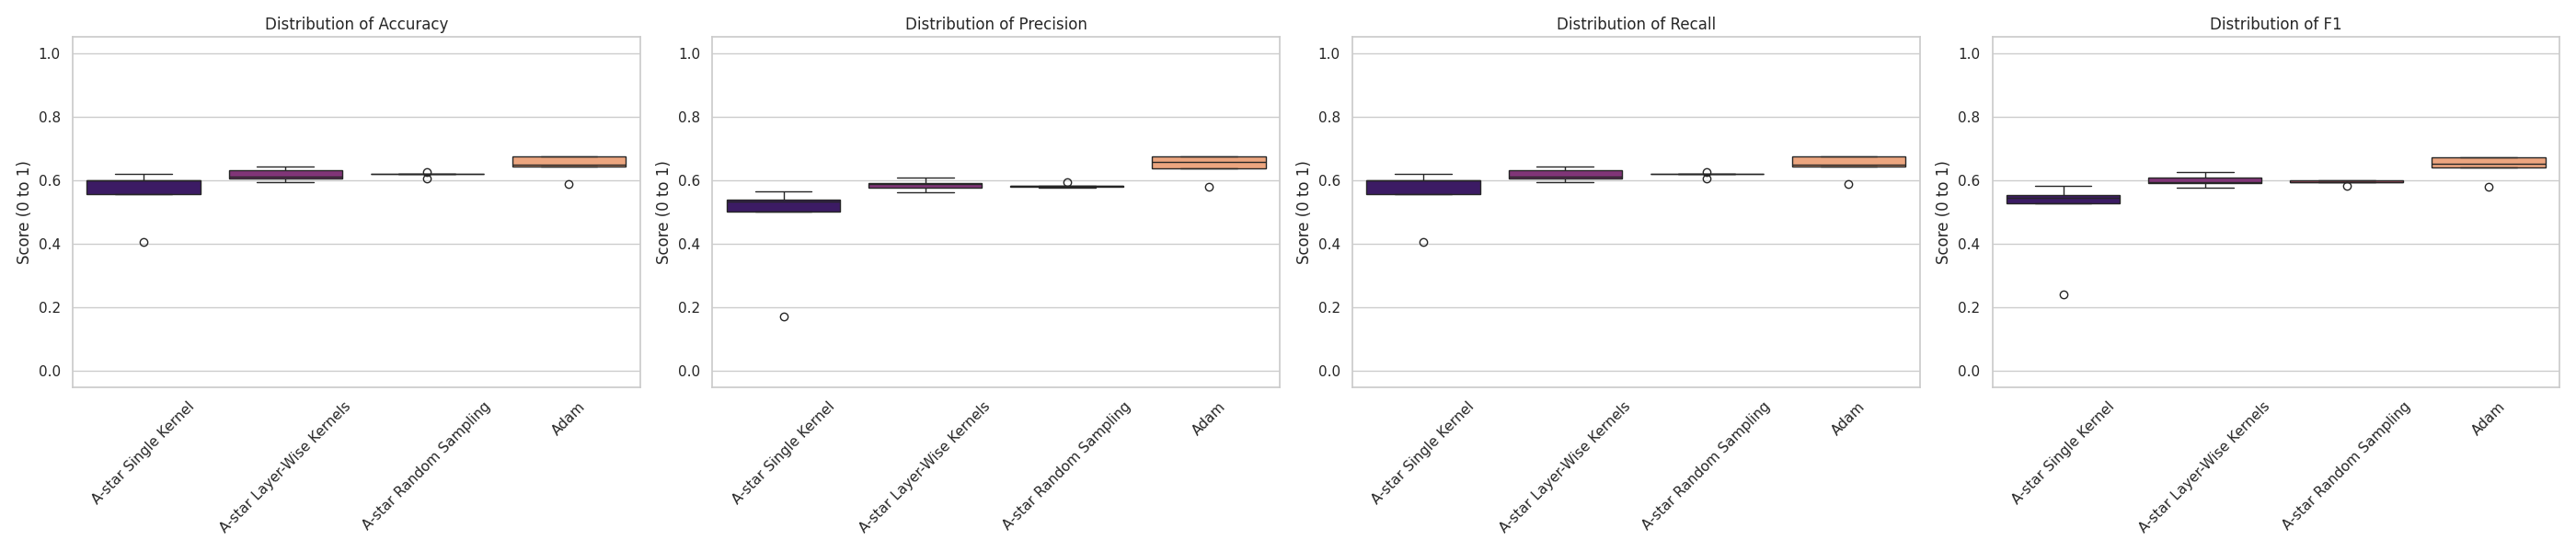
\includegraphics[width=1.05\textwidth]{figures/results/big_net_wine_Adam_vs_A-star/big_net_wine_Adam_vs_A-star_classification_metrics.png}
    \caption{Classification metrics distribution for Big Net.}
    \label{fig:big_wine_metrics_dist}
\end{figure}

Adam maintains its lead on the test set with an accuracy of $0.6462$. However, the \textit{Layer-Wise} and \textit{Random Sampling} methods remain competitive at $0.6175$. The discrepancy between Adam’s near-zero training loss and its moderate test accuracy further supports the observation that the Wine dataset contains inherent noise or class overlap that resists perfect generalization, regardless of the optimization depth.

\subsubsection{Summary Statistics}

Table \ref{tab:big_net_wine} presents the numerical comparison.

\begin{table}[htbp]
\centering
\scriptsize
\begin{tabular}{|l|c|c|c|c|}
\hline
\textbf{Metric}   & \textbf{$A^*$ Single Kernel} & \textbf{$A^*$ Layer-Wise} & \textbf{$A^*$ Random} & \textbf{Adam} \\ \hline
\multicolumn{5}{|l|}{\textit{Metrics computed on Training Set:}} \\ \hline
Avg Final Loss          & 1.044150                     & 0.792313                  & 0.852458              & \textbf{0.009494} \\ 
Median Final Loss       & 0.954967                     & 0.793027                  & 0.851581              & \textbf{0.007023} \\
Std Final Loss          & 0.130304                     & \textbf{0.007572}         & 0.015224              & 0.006161      \\ \hline
Avg Time (s)            & 2501.4289                    & 4960.8045                 & 3386.8323             & \textbf{15.4255}  \\ \hline
\multicolumn{5}{|l|}{\textit{Metrics computed on Test Set:}} \\ \hline
Avg Accuracy            & 0.556250                     & 0.617500                  & 0.617500              & \textbf{0.646250} \\ 
Avg Precision           & 0.462462                     & 0.585682                  & 0.582904              & \textbf{0.645187} \\ 
Avg Recall              & 0.556250                     & 0.617500                  & 0.617500              & \textbf{0.646250} \\ 
Avg F1                  & 0.490386                     & 0.599217                  & 0.594114              & \textbf{0.642548} \\ \hline
\end{tabular}
\caption{Average statistical comparison on Wine Quality - Big Net.}
\label{tab:big_net_wine}
\end{table}

\subsection{Conclusions on Wine Quality Benchmark}

The Wine Quality benchmark highlights the boundaries between gradient-based and discrete search optimization:

\begin{itemize}
    \item \textbf{Gradient Dominance in Complex Classification:} Unlike the Iris benchmark where $A^*$ reached absolute zero, the Wine dataset seems to be a more complex landscape where Adam’s gradient-based updates are significantly more effective at escaping high-loss plateaus.
    \item \textbf{Search Stability:} While $A^*$ methods struggled to match Adam's final depth, they demonstrated superior stability (lower variance) in the Medium and Big net regimes, particularly the Layer-Wise kernel strategy.
    \item \textbf{Implicit Regularization:} The "stagnation" of $A^*$ methods at higher training losses did not lead to a catastrophic drop in test accuracy, suggesting that discrete search naturally avoids some of the sharpest training minima that might otherwise lead to overfitting in noisy datasets.
\end{itemize}